\begin{artplenv}{Wojciech Rybka}
	{Problem istoty i~pomiaru dobrobytu}
	{Problem istoty i~pomiaru dobrobytu}
	{Problem istoty i~pomiaru dobrobytu}
	{Uniwersytet Ekonomiczny w~Krakowie\label{rybka-start}}
	{The problem of the essence and measurement of well-being}
	{Well-being is becoming an increasingly popular issue in economics. The aim of the article is to present the concept of well-being and the methods of its measurement and to examine the statistical significance between the results obtained by specific indicators. The article was written based on the meta-analysis of the books and scientific papers on the subject, as well as well-being and welfare measurement reports. The study shows that there is a~very wide range of theories and concepts related to well-being which are sometimes exceptive. The most important conclusion from the study is that the correlation between welfare and well-being represented respectively by GDP and HDI is very strong, while the correlation between welfare and life satisfaction as well as well-being and subjective well-being are negligible.}
	{well-being, welfare, quality of life, economics, philosophy of economics.}



\section*{Wstęp}
\lettrine[loversize=0.13,lines=2,lraise=-0.05,nindent=0em,findent=0.2pt]%
{H}{}istoria badań nad dobrobytem sięga starożytności. Już najwcześniejsi filozofowie zastanawiali się, jak żyć dobrze oraz
czym jest dobre życie. Na przestrzeni dziejów ludzie tworzyli różnorodne koncepcje, niekiedy znacznie się różniące.
Problematyka dobrobytu, dobrostanu czy jakości życia jest poruszana nie tylko przez przedstawicieli nauk społecznych,
ale także przez filozofów oraz medyków. Z~biegiem czasu tworzono różnego rodzaju klasyfikacje oraz wskaźniki próbujące
go zmierzyć. Pojęcie dobrobytu obecnie rozwijane jest głównie na terenie ekonomii. Historia myśli ekonomicznej
odnotowuje wiele teorii oraz wskaźników odnoszących się do jego różnych wymiarów.

W niniejszym artykule przedmiotem analizy są koncepcje dobrobytu, kwestie ich pomiaru oraz istotność statystyczna
korelacji pomiędzy wynikami pomiarów. Autor postawił sobie za zadanie rozróżnienie oraz wskazanie różnorodności teorii
dobrobytu stosowanych w~ekonomii oraz innych naukach, przedstawienie wskaźników umożliwiających ich pomiar oraz
obliczenie zależności pomiędzy wartościami reprezentowanych przez nie wskaźników. Celem pracy jest także analiza zmian
dobrobytu zachodzących w~Polsce oraz Grecji. 

Artykuł podzielony jest na cztery części. Pierwsza z~nich ukazuje historię związaną z~koncepcjami dobrobytu występującymi
w~naukach ekonomicznych, filozofii oraz innych dyscyplinach naukowych. W~tej części przedstawiono i~rozwinięto
najważniejsze teorie dobrobytu występujące w~wymienionych dziedzinach. Wskazano także proces ewolucji pojęciowej
wraz z~przedstawieniem jego przyczyn.

Druga część ukazuje wskaźniki mierzące różne odmiany dobrobytu. Określa także~ich mocne i~słabe strony oraz
szanse i~zagrożenia związane z~ich stosowaniem. Celem tej części pracy jest przedstawienie kompleksowego przekroju przez
historię pomiarów dobrobytu w~ekonomii oraz ukazanie ich ewolucji na przestrzeni wieków. Fragment ten ma także
przybliżyć czytelnikowi czynniki, które brane są pod uwagę przy tworzeniu wskaźników oraz ukazanie ich różnorodności.
Autor zwrócił szczególną uwagę na produkt krajowy brutto, który jest najpopularniejszym miernikiem dobrobytu
ekonomicznego. W~dalszej części pracy autor przedstawił i~opisał wskaźniki uzupełniające, regulujące oraz alternatywne
wobec PKB.

Trzecia część artykułu poświęcona jest pomiarom poszczególnych wymiarów dobrobytu przez różne wskaźniki oraz skale.
Autor pracy analizuje związek statystyczny pomiędzy dobrobytem ekonomicznym, ogólnym oraz subiektywnym obliczany
odpowiednio przez wskaźniki PKB, HDI oraz SWB. Fragment ten zawiera także szczegółową analizę zmian wartości wskaźników
zachodzących w~wybranych krajach oraz próbę wyjaśnienia przyczyn tych zmian. Do analizy wartości otrzymanych przez
wskaźniki autor użył metod statystycznych.

Ostatnia część stanowi zakończenie, w~którym znajduje się podsumowanie pracy  i~przeprowadzonych badań oraz zalecenia
autora co do przyszłych badań nad zagadnieniem dobrobytu.

Autor podjął się analizy koncepcji dobrobytu oraz zależności zachodzących pomiędzy wynikami ich pomiaru, ponieważ
tematyka ta, tak samo jak filozofia ekonomii, zyskuje na popularności w~opracowaniach polskich i~zagranicznych. Drugą
przesłanką do wyboru tego tematu jest niedokładność definicyjna stosowana w~polskich opracowaniach, która prowadzi do
niejasności i~pomyłek w~opracowaniach.

\section{Zagadnienie dobrobytu w~filozofii i~ekonomii}
\vskip-2\baselineskip
\subsection{1.1. Ekonomiczne ujęcie dobrobytu}
Dobrobyt w~ekonomii ujmowany był w ramach różnych koncepcji, które ulegały ewolucji na przestrzeni czasu. Ekonomiści (głównie
neoklasycy) utożsamiali dobrobyt z~użytecznością pewnego koszyka dóbr i~usług
\parencite{kot_dobrobyt_2004}.
%\label{ref:RND6VH6PmWfV2}(Kot, i~in., 2004).
W metryce pieniężnej jest on rozumiany jako użyteczność dochodu koniecznego do zakupu danych dóbr i~usług.
Zgodnie z~tą koncepcją przyjmuje się, że im większy jest dochód, tym większy jest dobrobyt (użyteczność dochodu,
zamożność). Mimo tego, że teoria ta przeszła w~ekonomii długą  i~burzliwą ewolucję, to nadal utożsamiana
jest z~pojęciami materialnymi, a~nie stopniem zadowolenia z~życia czy szczęścia. Dla współczesnych ekonomistów coraz bardziej
oczywisty staje się pogląd, że utylitarystyczna podstawa dobrobytu jest niewystarczająca. Według Amartyi Sena jest on
czymś więcej niż zamożnością ekonomiczną. Uważa on dobrobyt ekonomiczny za narzędzie do osiągania dobrobytu, a~nie cel
sam w~sobie. 

W literaturze ekonomicznej do określenia dobrobytu stosuje się dwa terminy. Są to pochodzące z~języka angielskiego
wyrażenia \textit{well-\mbox{-being}} oraz \textit{welfare}. Termin \textit{well-being} jest utożsamiany z~koncepcją ogólnego
dobrobytu, a~\textit{welfare} z~dobrobytem ekonomicznym (zamożnością)
\parencite{kot_dobrobyt_2004}.
%\label{ref:RND1h4RYYJd2Q}(Kot, i~in., 2004).
%Dobrobyt ogólny rozumiany jest także jako odczuwalny stan zdrowia oraz szczęścia
%\parencite{noauthor_well-being_2019}.
%\label{ref:RNDcJeLoRYp6q}(Well-Being, 2019).
Dobrobyt ogólny, rozumiany także jako odczuwalny stan zdrowia oraz szczęścia
\parencite{noauthor_well-being_2019}, nawiązuje do filozoficznej koncepcji dobrostanu.
%Definiuje on dobrobyt w~pozadochodowych aspektach, nawiązując do filozoficznej koncepcji dobrostanu.
Ekonomia
neoklasyczna mianem dobrobytu określa dobrobyt ekonomiczny. Różnica pomiędzy tymi dwoma pojęciami jest
zauważalna w~literaturze anglojęzycznej. W~polskich opracowaniach (także w~przekładach z~języka angielskiego) wyrażenia te
traktowane są jako synonimy  i~tłumaczone jednym słowem -- dobrobyt. Jest to bardzo mylące zawężenie pojęciowe, ponieważ
miesza ono dwie różne od siebie koncepcje. Zabieg ten zaciera granicę między tymi pojęciami -- nie tylko terminologiczną,
ale także znaczeniową.

Odrzucenie koncepcji ogólnego dobrobytu w~teorii ekonomii tłumaczy Vilfredo Pareto. Według niego \textit{homo
oeconomicus} jest tylko cząstką natury człowieka żyjącego  i~funkcjonującego w~znacznie szerszym niż ekonomia
kontekście społecznym. Jego zdaniem, ekonomia nie może służyć do rozstrzygania problemów społecznych, ponieważ jej
zadaniem jest prowadzenie badań oraz stawianie postulatów z~zakresu zaspokajania ekonomicznych preferencji jednostek.
Zdaniem Pareto, użyteczność (społeczna lub indywidualna) jest pochodną innych czynników, które należą do zainteresowań
filozofii, socjologii czy etyki. Według niego ekonomiści nie posiadają w~zakresie swojej dziedziny kryteriów oraz
narzędzi pozwalających na przeprowadzenia takich analiz
\parencite{czech_ekonomia_2014}.
%\label{ref:RNDgi5V6Ffk5h}(Czech, 2014).

W ekonomii głównego nurtu indywidualny dobrobyt rozumiany był jako użyteczność pochodząca z~konsumpcji dóbr i~usług.
Jest ona traktowana jako numeryczna reprezentacja konsumenckiego wyboru, zgodna z~teorią preferencji ujawnionych
\parencites{boehm_is_2002}{ostapiuk_droga_2019}.
%\label{ref:RND6kRFXHPUSR}(Mongin, 2002; zob. także Ostapiuk, 2019).
Dobrobyt jednostkowy jest interpretowany także jako
stan psychiczny -- taki dobrobyt nazywa się dobrobytem subiektywnym. Ekonomiści w~tym przypadku posługują się badaniami
sondażowymi, zawierającymi pytania o~subiektywną ocenę własnego dobrobytu, pozwalającą ocenić użyteczność otrzymywanego
dochodu
\parencite{kot_ekonometryczne_2000}
%\label{ref:RND3AEtRWbL8h}(Kot, 2000)
lub poziom szczęścia
\parencite{blanchflower_well-being_2004}.
%\label{ref:RNDid4lYzkFcS}(Blanchflower, Oswald, 2004).
Sen uważa, że reprezentacja wyborów konsumenta nie zawsze obrazuje poziom jego dobrobytu, ponieważ
kupujący kierują się także motywami innymi niż troska o~własny byt
\parencite{zaremba_dobrobyt_2016}.
%\label{ref:RNDbQusAffsdF}(Zaremba, 2016).
Także
dochód i~konsumpcja nie są według niego dobrymi miarami dobrobytu. Dochód o~danej wielkości odpowiadać może różnym
poziomom dobrobytu, ponieważ jest to wartość \textit{stricte} subiektywna. 

Zwiększająca się popularność zagadnienia dobrobytu i~jego liczne koncepcje spowodowały powstanie odrębnej
dziedziny w~ekonomii, czyli ekonomii dobrobytu (\textit{welfare economics}). Warto wspomnieć,
że przedmiotem jej zainteresowań jest
\textit{homo oeconomicus}, czyli podmiot, który maksymalizuje swoją użyteczność (satysfakcję) dzięki zaspokajaniu
własnych, niezmiennych w~czasie preferencji konsumenckich. Ekonomia dobrobytu z~biegiem czasu stała się integralną
częścią klasycznej szkoły ekonomii. 

Pierwszym teoretycznym dziełem ekonomii dobrobytu była publikacja Arthura Pigou  \textit{Wealth and Welfare
[Bogactwo i~dobrobyt]}
\parencite*{pigou_wealth_1912}.
%\label{ref:RNDLKGPhide3U}(1912).
Została ona następnie rozszerzona i~wydana pod tytułem \textit{The
Economics of Welfare [Ekonomia Dobrobytu]}
\parencite*{pigou_economics_1920}.
%\label{ref:RNDT12Fu6D2x7}(1920).
Prace te usankcjonowały oficjalną nazwę tej
dyscypliny oraz stały się podstawą określonej orientacji teoretycznej. Zawarte zostało w~nich rozróżnienie pomiędzy
pozyskiwaniem satysfakcji z~zaspokajania potrzeb (\mbox{\textit{needs}}) oraz pragnień (\textit{desires})
\parencite{czech_ekonomia_2014}.
%\label{ref:RNDsWeO2W26RW}(Czech, 2014).
Pierwsze z~nich wiążą się z~obiektywnie określonymi, podstawowymi potrzebami
człowieka (m.in. higieną, odżywianiem, edukacją, odpoczynkiem). Drugie natomiast nawiązują do spełniania ludzkich
pożądań i~zachcianek (w~tym kontekście pożądanie oznacza silne, długotrwałe pragnienie danej rzeczy, a~zachcianka to
chwilowa, łatwo zmieniająca się ochota na coś)
\parencite{czech_ekonomia_2014}.
%\label{ref:RND1XYB7nX5cQ}(Czech, 2014).

Współczesna ekonomia dobrobytu określana jest jako podstawa polityki społeczno-gospodarczej państwa. Zajmuje się ona
poprawą efektywności alokacji zasobów, w~celu zmaksymalizowania zagregowanego dobrobytu społecznego. Rozważa
zagadnienia konstrukcji optymalnego systemu podatkowego, czy sposobu organizowania sprawnej gospodarki.

Definicja dobrobytu społecznego, tak samo jak jednostkowego, z~biegiem czasu ulegała ewolucji. W~ekonomii neoklasycznej
dobrobyt społeczny stanowił sumę użyteczności dochodów indywidualnych jednostek w~społeczeństwie
\parencite{zaremba_dobrobyt_2016}.
%\label{ref:RNDwe0Ev2B4Nk}(Zaremba, 2016).
Pigou dowodził, że społeczeństwo jest bliższe optimum
dobrobytu w~momencie, gdy dochód narodowy jest stabilny, wysoki oraz sprawiedliwie podzielony, a~podział ten związany musi być
głównie z~polityką podatkową państwa
\parencite{zaremba_dobrobyt_2016}.
%\label{ref:RNDGhHYEoBuXe}(Zaremba, 2016).

W opracowaniach, ekonomiści termin ,,pragnienie'' zastępują kategorią ,,preferencje''. Nie jest to jedynie terminologiczna
zmiana. W~przeciwieństwie do pragnień preferencje mają porównawczy charakter. Można to zilustrować przykładem: jeżeli
dana jednostka stoi przed wyborem jednej spośród dwóch opcji X lub Y, to może preferować tylko jedną z~nich,
w~sytuacji, gdy pragnąć może dwóch naraz
\parencite{kwarcinski_koncepcje_2016}.
%\label{ref:RND68upEwQ8VH}(Kwarciński, 2016).
Zwolennicy koncepcji
preferencji ujawnionych uważają,
że preferencje jednostek są ujawniane poprzez dokonywanie wyborów. W~sytuacji, gdy dana jednostka
stoi przed wyborem kupna roweru lub skutera i~wybiera rower oznacza to, że preferuje pierwszą opcję. 

Pojęcie dobrobytu w~naukach ekonomicznych utożsamiane jest głównie (dzięki ekonomii neoklasycznej) z~dobrobytem
ekonomicznym. Przez dziesięciolecia rozważań na jego temat, w~literaturze powstało wiele koncepcji
rozszerzających i~uzupełniających jego pierwotne znaczenie. Z~biegiem czasu teorią dobrobytu
zajmowały się także inne dziedziny naukowe, w~tym filozofia. Rozważa ona głównie pozaekonomiczne
aspekty oraz czynniki mogące prowadzić do jego wzrostu. 

\subsection{1.2. Filozoficzne ujęcie dobrobytu}
W filozofii pojęcie dobrobytu zostało zaczerpnięte z~nauk ekonomicznych. Dlatego rozważania na jego temat mają
stosunkowo krótką historię. Jednakże już od starożytności filozofowie zastanawiali się nad dobrostanem i~zadawali sobie
pytania o~dobre życie. Wyróżnili oni -- podobnie jak później w~ekonomii -- dwa wymiary: jednostkowy i~społeczny. Należy
pamiętać, że filozofia zajmuje się głównie pojęciem dobrobytu ogólnego jednostki oraz społeczeństwa
(\textit{well-being}) -- w~tej części termin ,,dobrobyt'' oznaczać będzie koncepcję dobrobytu ogólnego. 

Filozoficzne ujęcie dobrobytu (dobrostanu, dobrego życia) związane jest z~pytaniami ,,co jest dobre dla człowieka?'' oraz
,,jakie życie jest dla człowieka dobre?''. Filozofia ujmuje również problem od strony negatywnej wskazując, co jest dla
jednostki złe. Filozofowie patrzą głównie na życie człowieka jako całość jego istnienia, a~nie jedynie poszczególne
jego fragmenty. 

Koncepcje dobrobytu były ważnym motywem prac Arystotelesa. Zadawał on pytania o~dobre życie,
a~jego rozwiązania reprezentują pogląd zwany eudajmonizmem,
zgodnie z którym szczęście danej osoby stanowi najwyższą wartość i~ostateczny cel ludzkiego
życia. Eudajmonizm rozumie szczęście nie jako subiektywne zadowolenie, lecz jako stan zachodzący wskutek właściwego
postępowania
\parencite{moleda_kantowska_2009}.
%\label{ref:RNDJ4IzCcvV2g}(Molęda, 2009). 

W filozofii XVIII i~XIX wieku dobrobyt stanowił centrum zainteresowań filozofów Jeremy'ego Benthama oraz Johna Stuarta
Milla. Reprezentowali oni nową wersję hedonizmu, która była przez nich traktowana jako część teorii utylitarystycznej
\parencite{brey_well-being_2012}.
%\label{ref:RNDdLyKmevkGd}(Brey, 2012).
We współczesnych rozważaniach filozoficznych dobrobyt ponownie stał się ważnym
tematem, który zyskał znaczną popularność w~ostatnich trzydziestu latach.

Derek Parfit, jeden ze znanych współczesnych filozofów, w~swojej książce \textit{Racje i~osoby}
\parencite*{parfit_racje_2012}
%\label{ref:RNDlZoiUoryXX}(2012)
zadaje pytanie, ,,co byłoby dla kogoś najlepsze, najbardziej leżało w~jego interesie
albo czyniło jego (jej) życie w~jego (jej) własnych oczach tak dobrym, jak tylko możliwe?''. Odpowiedzi na to pytanie
nazywa \textit{teoriami na temat interesu własnego}. Zostały one także rozwinięte w~pracach Jamesa Griffina oraz
Leonarda Sumnera. 

Do głównych teorii dobrobytu filozofowie zaliczali
\parencite{brey_well-being_2012}:
%\label{ref:RNDer2t8feRbG}(Brey, 2012):

\begin{itemize}
\item hedonizm,
\item teorię zaspokajania pragnień,
\item teorię listy dóbr obiektywnych.
\end{itemize}

Pierwsza z~teorii głosi, że przyjemność jest wewnętrznie dobra a~ból jest wewnętrznym złem. Według niej dana jednostka
wiedzie dobre życie wtedy, gdy dąży do przyjemności, a~unika bólu. Dążenie do dobrobytu to dążenie do jak największej
ilości przyjemności oraz jak najmniejszej ilości bólu (cierpień). Wcześniejsze formy hedonizmu wywodzą się z~czasów
starożytnych. W~swoich tekstach Epikur głosił, że dobre życie jest możliwe do osiągnięcia wtedy, gdy człowiek
maksymalizuje przyjemność i~unika przedłużającego się strachu oraz cierpienia cielesnego. 

Bentham oraz Mill byli zwolennikami dwóch różnych rodzajów hedonizmu. Pierwszy z~nich optował za tzw. ilościowym
hedonizmem. Uważał on, że wartość przyjemności zależy wyłącznie od ilości, a~nie od jej jakości. Nie ma
znaczenia w~takim razie jej rodzaj czy też źródło. W~swojej książce pisze: ,,Natura poddała rodzaj ludzki rządom dwu zwierzchnich
władców: przykrości i~przyjemności. Im tylko dane jest wskazywać, cośmy powinni czynić oraz stanowić o~tym, co będziemy
czynili''
\parencite[s.~17]{bentham_wprowadzenie_1958}.
%\label{ref:RNDewCktqXyPy}(Bentham, 1958, s. 17).
Od samego początku publikacja wywołała kontrowersje. Mill był
zwolennikiem hedonizmu jakościowego. Twierdził on, że niektóre przyjemności są cenniejsze lub przyjemniejsze niż inne.
W~swoim dziele pt. \textit{Utylitaryzm} pisał: ,,lepiej być niezadowolonym człowiekiem, niż zadowoloną świnią; lepiej
być niezadowolonym Sokratesem, niż zadowolonym głupcem''
\parencite[s.~18]{mill_utylitaryzm:_1959}.
%\label{ref:RNDYZ2bdeVALU}(Mill, 1959, s. 18).

\enlargethispage{1\baselineskip}

Drugą koncepcją zaliczaną do teorii na temat interesu własnego jest teoria zaspokajania pragnień. Jej zwolennicy
utrzymują, że dobrobyt polega na zaspokajaniu pragnień jednostki. Koncepcja ma swój początek w~XIX
wieku w~opracowaniach ekonomii dobrobytu. Ówcześni ekonomiści chcieli, aby koncepcja miała obiektywne kryteria w~pomiarze
dobrobytu oraz użyteczności jednostek. Jednakże przyjemność i~cierpienie znajdują się w~umysłach ludzi, dlatego nie
mogą być łatwo zmierzone. Z~tego względu ekonomiści reprezentujący to stanowisko nie skupiają się na mentalnych stanach
podmiotów. Uważają, że ludzie zwykle są w~stanie ocenić własne preferencje i~uszeregować je względem siebie. Pozwala to
na utworzenie funkcji użyteczności, których wartość jest związana z~zaspokojeniem preferencji.

Trzecia koncepcja wchodząca w~skład teorii na temat interesu własnego to koncepcja listy dóbr obiektywnych.
Zgodnie z~jej zasadą pewne rzeczy są dobre albo złe dla ludzi, bez względu na to, czy faktycznie osoby chciałyby dobre rzeczy
posiadać, a~unikać tych złych. To znaczy, że istnieją rzeczy obiektywnie dobre dla ludzi, nawet gdy ich nie pożądają.
Takimi rzeczami są np. wykształcenie, wolność słowa, zdrowie
\parencite{mill_utylitaryzm:_1959}.
%\label{ref:RNDWrM4KkB4rX}(Mill, 1959).
Wśród rzeczy złych
mogłyby znajdować się np. zdrada, bycie szkalowanym, manipulowanym, oszukiwanym czy też pozbawionym wolności. 

Lista dóbr obiektywnych przeciwstawia się hedonizmowi, podkreślając stany świata, a~nie mentalne stany podmiotu.
Staje w~opozycji do koncepcji zaspokajania pragnień twierdząc, że wartości stanów świata są niezależne od pragnień jednostki.
Parfit
\parencite*{parfit_racje_2012}
%\label{ref:RNDaqPqHfiJiI}(2012)
twierdzi, że hedonizm i~koncepcja zaspokajania pragnień mają deskryptywny
charakter, natomiast lista dóbr obiektywnych jest koncepcją wartościującą.

\enlargethispage{1\baselineskip}

Hedonizm, teoria zaspokajania pragnień oraz lista dóbr obiektywnych są od pewnego czasu trzema głównymi, rywalizującymi
między sobą, filozoficznymi koncepcjami dobrobytu. Niektórzy próbowali rozwiązać spór pomiędzy nimi, łącząc dwie lub
trzy ze sobą, tworząc koncepcje hybrydowe. Jednym ze sposobów stworzenia wersji hybrydowej jest włączenie przyjemności
albo zaspokajania preferencji do listy dóbr obiektywnych. Inną możliwością jest stwierdzenie, że niektóre pragnienia
odpowiadają obiektywnym potrzebom
\parencite{hamilton_political_2003}.
%\label{ref:RNDVSDcVeCgGf}(Hamilton, 2003).
Jeszcze innym podejściem jest
argumentowanie, że teoria zaspokajania pragnień albo świadomy jakościowy hedonizm doprowadziłby do wyboru pozycji
znajdującej się na liście dóbr obiektywnych lub sugestia, że elementy z~listy są względne w~stosunku do osób czy
okoliczności. Zabiegi te niwelują różnicę pomiędzy trzema koncepcjami.

\section{Sposoby pomiaru dobrobytu}
\vskip-2\baselineskip
\subsection{2.1. Problemy związane z~pomiarem dobrobytu}
Pomiar osiągnięć społecznych i~dokonań gospodarczych jest jednym z~najważniejszych zagadnień w~teorii ekonomii oraz
praktyce gospodarczej. Kwestia ta nie znajduje jednak~w pełni satysfakcjonującego rozwiązania oraz w~miarę rosnącej
złożoności powiązań społeczno-gospodarczych i~postępu globalizacji coraz bardziej się komplikuje. Dlatego toczą się
debaty  i~badania ukierunkowane na poszukiwanie nowych miar rozwoju społecznego i~wzrostu gospodarczego. Wzrost
gospodarczy jest relatywnie prosty do pomiaru, ponieważ charakteryzuje go wymiar ilościowy. Lecz znacznie więcej
problemów przysparza pomiar rozwoju społeczno-gospodarczego. Składają się na niego m.in. wzrost gospodarczy, sytuacja
ekonomiczna oraz poprawa jakości życia społecznego. Sposób pomiaru, jego dokładność i~poprawność bywają problematyczne,
co może prowadzić w~dalszej konsekwencji do nieprawidłowości w~funkcjonowaniu społeczeństwa i~gospodarki
\parencite{cieslik_dylemat_2014}.
%\label{ref:RNDHyuxHBAOij}(Mączyńska, 2014).

Dobrobyt ekonomiczny (\textit{welfare}) oraz dobrobyt ogólny (\textit{well-\mbox{-being}}) także są przedmiotami pomiarów
ekonomicznych. Pierwszy z~nich związany jest ze wzrostem gospodarczym, a~drugi z~rozwojem społeczno-gospodarczym.
Jednak są to tylko dwie z~szerokiej gamy koncepcji dobrobytu, które znajdują się w~naukach ekonomicznych.

Niektóre z~koncepcji dobrobytu nie są kwantyfikowalne oraz mierzalne, szczególnie te o~charakterze jakościowym.
Uniemożliwia to dokonanie pomiaru, obliczenie średniej dla danego kraju, a~nawet porównania interpersonalne. Dane
jakościowe, które otrzymuje się m.in. przez wywiady, dostarczają pogłębionych informacji na dany temat. Do pomiaru
dobrobytu korzysta się jednak głównie z~danych ilościowych, które nie ujmują przyczyn danego zjawiska. Stosowanie
wyłącznie danych ilościowych wpływa na precyzję otrzymywanych wyników oraz ich zgodność z~rzeczywistością.

Problemem w~pomiarze dobrobytu subiektywnego jest także czynnik ludzki, respondent bowiem nie zawsze jest kompetentnym
sędzią w~swojej sprawie. Odpowiedzi dotyczące zadowolenia z~życia czy też postrzegania
jego jakości mogą różnić się w~zależności
od nastroju badanego i~nie będą adekwatnie odnosić się do całokształtu życia. Na przykład w~momencie, gdy zapytana
osoba będzie w~dobrym humorze, stopień zadowolenia będzie wyższy niż w~sytuacji złego samopoczucia. 

\subsection{2.2. PKB jako podstawowy miernik dobrobytu}
Prowadzenie rachunków narodowych ukazujących dokonania gospodarcze krajów ma bardzo długą historię. Już w~czasach
starożytnej Grecji działalność gospodarcza była przedmiotem rozważań. W~tamtym okresie powstało pojęcie ,,nadwyżki
ekonomicznej''. Kolejnym ważnym etapem w~rozwoju rachunków narodowych były poglądy merkantylistów. Zwracali oni uwagę na
handel i~eksport, a~za główne źródło bogactwa uważali obrót, w~którym eksport dóbr przewyższa import. Za prekursora
myśli makroekonomicznej i~koncepcji rachunków narodowych uważa się François Quesnay'a. W~roku 1758 opracował on
,,tablicę ekonomiczną'', będącą pierwszym w~historii myśli ekonomicznej schematem produkcji prostej i~pierwszym
prototypem rachunku narodowego. Następną ważną postacią był Adam Smith. Uważał on, że każda praca stanowi źródło
powstawania wartości, a~praca najemna przynosi wartość dodatkową. Wprowadził także pojęcie kosztów produkcji oraz
sformułował dogmat, który został nazwany później ,,dogmatem Smitha''. Według niego wartość rozkłada się na zyski, płace
i~rentę. Był to odpowiednik dzisiejszych dochodów czynników produkcji, do których zalicza się: pracę, kapitał oraz
ziemię. Kolejny kamień milowy stanowiły prace Karola Marksa, w~których opracował koncepcję schematów reprodukcji. Nie
można także zapomnieć o~postaci Wasyla Leontiefa, z~którą wiążą się tablice przepływów międzygałęziowych
(\textit{input/output}). Także w~Polsce, w~okresie międzywojennym ekonomiści Michał Kalecki oraz Ludwik Landau
stworzyli nowatorski szacunek dochodu narodowego Polski
\parencite{zienkowski_co_2001}.
%\label{ref:RNDkzvKN1pPEK}(Zienkowski, 2001).

Kamieniem milowym było sformułowanie w~latach 30. XX wieku najpowszechniejszego obecnie i~fundamentalnego rachunku
narodowego, jakim jest produkt krajowy butto. Jego nowoczesną wersję opracował Simon Kuznets dla raportu Kongresu
USA z~1934 roku. W~tym samym raporcie ostrzegł on przed jego wykorzystaniem jako miary dobrobytu ekonomicznego
\parencite{dickinson_gdp:_2011}.
%\label{ref:RND7xFAqFbE0Z}(Dickinson, 2011).

Wskaźnik ten odzwierciedla jednocześnie dwie wielkości: dochód całkowity wszystkich podmiotów będących częścią
gospodarki oraz sumę wydatków na dobra i~usługi. Określa on łączną wartość różnego typu produktów jako ogólny miernik
poziomu aktywności gospodarczej. Wykorzystuje się do tego ceny rynkowe, czyli kwotę, którą ludzie są w~stanie zapłacić
za dane dobro. PKB jest obszernym miernikiem obejmującym wszystkie dobra i~usługi, które wytwarzane są w~danej
gospodarce, a~później sprzedawane legalnie na rynku.

Produkt krajowy brutto jest jednak wyłącznie miernikiem, wyznacznikiem produkcji rynkowej. Mimo tego, że jest podstawą
oraz składnikiem wielu wskaźników, nie przekłada się on wprost na poziom krajowego bogactwa oraz społecznego
dobrobytu -- i~to pomimo tego faktu, że jest ważną składową jego kształtowania. Nie obejmuje on rezultatów pozarynkowych działań i~prac,
w tym m.in. prac wykonywanych samodzielnie w~domu. Dlatego także jako miernik postępu
społeczno-gospodarczego i~dobrostanu oraz dobrobytu społecznego kraju zawodzi, ponieważ
jest niewystarczający do kompleksowej oceny dokonań w~danym zakresie.
Produkt krajowy brutto jest twardym pomiarem ilościowym nieuwzględniającym ważnych aspektów, takich jak
jakość życia, estetyka czy spokój. Są to miękkie wartości, których nie można wycenić
\parencite{dickinson_gdp:_2011}.
%\label{ref:RNDfhz8Pbmn8G}(Dickinson, 2011).

Jak zostało wcześniej przedstawione, PKB stanowi wskaźnik dobrobytu ekonomicznego. Reprezentuje on łączne dochody
mieszkańców kraju oraz jednocześnie ich łączne wydatki na dobra i~usługi. Zaś PKB \textit{per capita} ukazuje informacje o
dochodach i~wydatkach statystycznego obywatela. Większość ludzi pragnie zarabiać więcej oraz więcej wydawać, dlatego
wskaźnik ten można zaliczać do mierników dobrobytu.

Popularność produktu krajowego brutto wynika także z~tego, że rozwój społeczny w~XX wieku był utożsamiany ze wzrostem
gospodarczym. We współczesnych społeczeństwach dobrobyt jest nadal postrzegany przez pryzmat ilościowych i~materialnych
wskaźników wzrostu gospodarczego. Obraz gospodarki kształtowany tylko poziomem wskaźnika PKB oraz jego fluktuacją
stwarza często odbiegający od codzienności wizerunek rzeczywistości, z~którą styka się społeczeństwo. Prowadzi to do
poczucia alienacji, szczególnie wśród uboższej i~słabiej wykształconej części społeczeństwa. Nieznajomość istniejącego
stanu rzeczy oraz uleganie populistycznym sloganom rodzi niechęć do uczestnictwa w~życiu społecznym
\parencite{dickinson_gdp:_2011}.
%\label{ref:RND7HXSo00QDy}(Dickinson, 2011).
Ekonomia neoklasyczna fetyszyzuje bogactwo i~pieniądz kosztem jakości życia
\parencite{samuelson_ekonomia._2008}.
%\label{ref:RNDdvfwdbGiAi}(Samuelson, Nordhaus, 2008).
Konsekwencją takiego stanowiska jest dewaluacja uznawanych norm
moralnych i~wartości, kreowanie za wszelką cenę gospodarczego wzrostu, brak poszanowania środowiska naturalnego oraz
narastanie nierówności społecznych. 

Najczęściej przytaczanymi zastrzeżeniami wobec PKB są
\parencite{stiglitz_blad_2013}:
%\label{ref:RNDE7TGfSbEuZ}(Stiglitz, i~in., 2013):

\begin{itemize}
\item wliczanie wydatków, które nie wpływają na wzrost dobrobytu,
\item pomijanie wartości duchowych,
\item brak uwzględnienia usług świadczonych przez środowisko naturalne,
\item ignorowanie społecznych nierówności,
\item występowanie trudności w~analizach porównawczych państw, 
\item nieuwzględnianie amortyzacyjnych odpisów od środków trwałych, 
\item pomijanie różnic w~cenach dóbr i~usług w~poszczególnych krajach,
\item traktowanie równorzędnie dóbr o~różnym poziomie użyteczności,
\item brak korelacji między wartością PKB a~stanem środowiska naturalnego,
\item nieuwzględnienie nierówności dochodowych w~danym kraju,
\item brak uwzględnienia wartości czasu wolnego,
\item nieuwzględnianie korzyści płynących z~konsumpcji dóbr użytku trwałego.
\end{itemize}

Wymienione powyżej zastrzeżenia do wykorzystywania PKB jako miernika dobrobytu mają różną siłę.
Nie należy jednak całkowicie rezygnować z~zastosowania PKB w~rachunkach narodowych. Jest on miernikiem
określającym aktywność gospodarczą, wielkość produkcji oraz wartości dodanej. Zaletą produktu krajowego brutto jest
jego niezależność od subiektywnych metod wyceny. Do jego zalet należy także zaliczyć czytelną procedurę pomiaru
elementów składowych oraz ustalanie przez rynek cen, za pomocą których wyrażane są wartości dóbr i~usług
\parencite{luszczyk_pomiar_2013}.
%\label{ref:RNDSSK4v1vUty}(Łuszczyk, 2013).

PKB ukazuje dobrobyt ekonomiczny (\textit{welfare}) związany tylko z~bogactwem i~pieniędzmi. Jest on stosowany do
pomiaru dobrobytu głównie przez przedstawicieli ekonomii neoklasycznej. Zauważono jednak, że pomiar dobrobytu samym
wskaźnikiem PKB nie wystarcza. Dlatego ekonomiści przy współpracy z~przedstawicielami innych nauk społecznych, takich jak
socjologia czy psychologia, konstruowali nowe wskaźniki, które odnosiły się do szerszej gamy czynników niż sam majątek. 

Joseph E. Stiglitz, Amartya Sen oraz Jean-Paul Fitoussi w~Raporcie Komisji ds. Pomiaru Wydajności Ekonomicznej i~Postępu
Społecznego
\parencite{stiglitz_blad_2013}
%\label{ref:RNDC16yhBNNvp}(Stiglitz, i~in., 2013)
(znanym bardziej jako publikacja pt. \textit{Błąd pomiaru.
Dlaczego PKB nie wystarcza}) przeanalizowali wskaźniki mierzące dobrobyt oraz dokonali ich klasyfikacji. Wyjściowym
wskaźnikiem jest tytułowe PKB, które zostało skrytykowane. Autorzy pozostałe mierniki podzielili na trzy kategorie:

\begin{itemize}
\item wskaźniki regulujące PKB,
\item wskaźniki uzupełniające PKB,
\item wskaźniki zastępujące PKB. 
\end{itemize}

\subsection{2.3. Wskaźniki regulujące PKB}

Wskaźniki regulujące PKB uwzględniają takie podejścia, które są pomijane przez tradycyjne miary wyników gospodarczych, takie jak PKB
czy krajowe stopy oszczędności. Zostały dostosowane poprzez uwzględnienie monetarnych czynników środowiskowych
oraz społecznych.

Do wskaźników regulujących PKB zalicza się m.in.:

\begin{itemize}
\item Miernik dobrobytu ekonomicznego (\textit{Measure of Economic Welfare, MEW}),
\item Miernik trwałego dobrobytu ekonomicznego (\textit{Index of Sustainable Economic Welfare, ISEW}),
\item Wskaźnik rzeczywistego postępu (\textit{Genuine Progress Indicator, GPI}).
\end{itemize}

Wskaźniki te, podobnie jak produkt krajowy brutto, odnoszą się do ekonomicznej koncepcji dobrobytu. Uwzględniają one
jedynie większą gamę czynników niż PKB, lecz nadal są to czynniki monetarne odnoszące się wyłącznie do bogactwa
społeczeństwa, pomijając inne ważne aspekty ludzkiej egzystencji.

\subsection{2.4. Wskaźniki uzupełniające PKB}
Drugą kategorią wskaźników opisanych w~raporcie są wskaźniki uzupełniające PKB. Zawierają one aspekty
pominięte w~obliczaniu PKB. Nie jest on w~nich regulowany przez dodatkowe monetarne czynniki, tylko dopełniany przez różne
niemonetarne, środowiskowe oraz społeczne dane. Są one jednak nadal oparte o~rachunki narodowe.

Do wskaźników uzupełniających PKB zalicza się m.in. wskaźniki zrównoważonego rozwoju oraz wskaźnik rozwoju społecznego
(\textit{Human Development Index, HDI}).

Zdefiniowane przez Eurostat wskaźniki zrównoważonego rozwoju służą do monitorowania realizacji celów strategii
zrównoważonego rozwoju Unii Europejskiej (\textit{European Union Sustainable Development Strategy}). Została ona
zatwierdzona w~2001 r. przez Radę Europejską podczas posiedzenia w~Göteborgu, następnie odnowiona w~czerwcu 2006~r.
Określa sposób, w~jaki Unia Europejska ma skutecznie sprostać wyzwaniom wiążącym się ze zrównoważonym rozwojem.
Dokument ten definiuje pożądane kierunki zmian w~perspektywie długookresowej w~sferach: gospodarczej,
ekologicznej i~społecznej, jak również sposoby ich osiągania. 

Wskaźnik rozwoju społecznego (HDI) to prawdopodobnie najbardziej znana próba podważenia hegemonii PKB w~rachunkowości
narodowej. Wskaźnik rozwoju społecznego został skonstruowany przez Organizację Narodów Zjednoczonych w~1990 r. Jego
podstawowym założeniem jest to, że ludzie są prawdziwym bogactwem narodu. Według jego twórców kluczowym celem rozwoju
jest stworzenie sprzyjającego środowiska oraz to, żeby ludzie mogli cieszyć się długim, zdrowym oraz twórczym życiem.
Wskaźnik HDI, w~przeciwieństwie do PKB, zakłada ekspansję dochodu narodowego jako środek do promocji rozwoju ludzkiego,
a~nie jako cel sam w~sobie. W~tym przypadku dochód uważany jest za konieczny, ale nie wystarczający warunek do
osiągnięcia społecznego rozwoju. Rozszerzony jest on o~dwie zmienne, czyli zdrowie oraz wykształcenie
\parencite{fioramonti_gross_2013}.
%\label{ref:RNDClmU8TrXre}(Fioramonti, 2013).
Sen, jeden z~twórców tego wskaźnika uważa, że indywidualne
możliwości są kluczowym elementem rozwoju człowieka. W~początkowej wersji wskaźnik rozwoju społecznego uwzględniał
następujące czynniki
\parencite{united_nations_development_programme_human_2019}:
%\label{ref:RND7MCVham9pF}(United Nations Development Programme, 2019):

\begin{itemize}
\item długie i~zdrowe życie mierzone oczekiwaną długością życia,
\item wiedzę mierzoną średnią liczbą lat edukacji oraz stopniem analfabetyzmu,
\item standard życia mierzony PKB \textit{per capita} liczonym według parytetu siły nabywczej.
\end{itemize}

Od samego momentu powstania wskaźnik ten jest szeroko stosowany przez naukowców oraz instytucje międzynarodowe,
szczególnie do analizy sytuacji w~mniej zamożnych krajach. HDI uwzględnia czynniki społeczno-ekonomiczne, lecz pomija
wolność polityczną i~prawa egzekwowane w~krajach. Takie podejście generuje paradoksy. Jednym z~nich jest fakt, że
Egipt, Libia oraz Tunezja, czyli kraje ogarnięte społecznymi buntami Arabskiej Wiosny w~2011 r., były konsekwentnie na
szczycie rankingu HDI krajów afrykańskich, a~wynikami dorównywały większości uprzemysłowionych narodów
\parencite{fioramonti_gross_2013}.
%\label{ref:RNDelLCkdjsXg}(Fioramonti, 2013).

Wraz z~upływem czasu HDI był modyfikowany. W~2010 roku wprowadzono wielorakie zmiany w~sposobie jego wyliczania.
Dotyczyły głównie dwóch wymiarów: zdrowia i~edukacji. Warto także zwrócić uwagę na rezygnację ze wskaźnika
piśmienności. Po raz pierwszy ONZ uznała, że analfabetyzm nie stanowi już światowego problemu. W~przypadku
edukacji i~zdrowia dokonano jedynie modyfikacji mierników, co spowodowało większą wrażliwość wskaźnika, która uwypukla różnice
pomiędzy krajami. Jednak największą zmianą jakiej dokonano jest to, że zamiast PKB \textit{per capita} liczonego parytetem siły
nabywczej używa się dochodu narodowego brutto (DNB). Zawiera on takie same wartości, jak produkt krajowy brutto oraz
dodatkowe informacje dotyczące salda dochodów zagranicznych. Powoduje to, że gospodarki o~dużym udziale zagranicznych
przedsiębiorstw będą miały niższe DNB niż PKB. Jak przyznają autorzy, kolejne reformy liczenia HDI będą skupiać
się w~większym stopniu na nierównościach w~rozwoju społecznym
\parencite{antczak_nowe_2012}.
%\label{ref:RND2pfZeWyV55}(Antczak, 2012).

%\enlargethispage{1\baselineskip}

Wskaźniki uzupełniające PKB odnoszą się do koncepcji ogólnego dobrobytu. Biorą one pod uwagę nie tylko czynniki
monetarne, związane z~dobrobytem ekonomicznym, ale także środowiskowe oraz społeczne. Jednakże definiują one tylko
rzeczy zewnętrznie wpływające na dobrostan ludzi. Nie uwzględniają czynników wiążących się z~poczuciem subiektywnego
dobrobytu.

\subsection{2.5. Wskaźniki zastępujące PKB}
Następująca kategoria wskaźników ma na celu zastąpienie PKB jako miary dobrobytu. Wskaźniki te biorą pod uwagę o
wiele szersze spektrum czynników mogących wpływać na dobrostan ludzi. Biorą one pod uwagę nie tylko pieniężne czynniki,
ale także m.in. społeczne, zdrowotne, środowiskowe oraz psychiczne. Wskaźniki zaliczane do tej grupy skupiają się
głównie na dobrobycie subiektywnym. Do grupy wskaźników zastępujących zalicza się m.in. światowy wskaźnik szczęścia
(\textit{Happy Planet Index}, HPI) oraz wskaźnik dobrobytu subiektywnego (\textit{Subjective Well-Being}, SWB).

Na oficjalnej stronie Happy Planet Index można przeczytać: ,,HPI mierzy to, co ważne: zrównoważony dobrobyt dla
wszystkich. Mówi o~tym, jak dobrze radzą sobie narody w~osiąganiu długiego, szczęśliwego i~zrównoważonego życia''
\parencite{noauthor_about_2019}.
%\label{ref:RND5EjiqveQ3W}(About the HPI, 2019).
Happy Planet Index został stworzony przez organizację New Economics
Foundation. Jest indeksem mierzącym dobrostan oraz wpływ ludzi na środowisko. Ma na celu zakwestionowanie PKB oraz HDI,
które są postrzegane jako wskaźniki nieuwzględniające zrównoważonego rozwoju. Indeks ten łączy w~sobie cztery elementy,
aby pokazać, jak efektywnie mieszkańcy korzystają z~zasobów środowiska, aby prowadzić długie i~szczęśliwe życie. Oblicza
się go według wzoru:

\begin{footnotesize}
\begin{widerequation}
\textit{HPI}\ {\approx}\ \frac{\textit{Średnia oczekiwana długość życia}\times\textit{Odczuwalny dobrostan}\times\textit{Nierówność wyników}}{\textit{Ślad ekologiczny}}
\end{widerequation}
\end{footnotesize}

Warto zwrócić uwagę na uwzględniony we wskaźniku ślad ekologiczny. Jest to wskaźnik, który pozwala na oszacowanie
zużycia zasobów naturalnych w~stosunku do możliwości ich odtworzenia przez Ziemię. Porównywana jest w~nim ludzka
konsumpcja zasobów naturalnych
\parencite{noauthor_about_2019}.
%\label{ref:RNDvhQx0fQ1FK}(About the HPI, 2019).

Światowy wskaźnik szczęścia wzbudza wiele kontrowersji. Jego przeciwnicy uważają, że nie mierzy on osobistego szczęścia
mieszkańców poszczególnych krajów, lecz ,,szczęście'' planety. Innymi słowy jest to miara ekologicznej efektywności
wspierania dobrobytu. Do plusów HPI można zaliczyć to, że posiada prosty do zrozumienia schemat wyliczania, jego dane
są łatwo dostępne oraz łączy ze sobą wykorzystanie zasobów naturalnych i~zdolności planety do ich regeneracji. Do
minusów należy zaliczyć niesystematyczność publikacji, nieaktualność niektórych danych składowych oraz, jak zostało
wcześniej wspomniane, fakt, że HPI nie mierzy dobrobytu ludzkiego, lecz jest miarą efektywności środowiskowej wspierania
dobrostanu w~danym kraju. 

Drugim wskaźnikiem alternatywnym wobec PKB jest SWB mierzony za pomocą skali zwanej Drabiną Cantrila. Została ona
utworzona przez Hadley'a Cantrila, który jest badaczem społecznym. Wykorzystywana jest w~badaniach pracowni sondażowej
Gallup World Poll oraz w~Happy Planet Index. Badanie polega na wypełnieniu ankiety przez respondenta, który ocenia pod
względem szczęśliwości swoje życie obecne oraz przyszłe
\parencite{krok_metody_2016}.
%\label{ref:RND66wMsg1fRT}(Krok, 2016).
Na początku badania
prosi się ankietowanego, aby wyobraził sobie drabinę ze szczeblami ponumerowanymi od 0 u~dołu do 10 u~góry. Szczyt
drabiny przedstawia najlepsze możliwe życie badanego, a~0 reprezentuje dla niego najgorsze możliwe życie. Następnie
dana osoba musi odpowiedzieć na dwa pytania
\parencite{gallup_inc._understanding_2019}:
%\label{ref:RNDAHBjpftqSZ}(Gallup Inc., 2019):

\begin{itemize}
	\item[--] Jak sądzisz, na którym stopniu drabiny szczęścia aktualnie się znajdujesz?
	\item[--] Jak sądzisz, na którym stopniu drabiny szczęścia będziesz się znajdował za 5 lat?
\end{itemize}

Pierwsze pytanie odnosi się do aktualnego szczęścia odczuwanego przez ankietowanego. Drugie zaś odnosi się do jego
przewidywanego poczucia szczęścia. Później oceny zebrane z~pierwszego oraz drugiego pytania łączy się w~celu poprawy
wiarygodności skali. 

Analizy statystyczne sugerują, że dwa elementy mierzą wspólny wymiar dobrobytu, ponieważ bardzo silnie ze sobą korelują,
tworząc niezależny i~wiarygodny wskaźnik. Dzięki temu, że bada się dwie perspektywy czasowe, zmniejsza się
prawdopodobieństwo, że odpowiedź o~całokształt odczuwanego dobrobytu będzie uwarunkowana aktualnym stanem zadowolenia
badanego.



Wskaźniki wymienione powyżej zaliczane są do wskaźników alternatywnych wobec PKB. HPI oraz SWB mierzą nie tylko
ekologiczne aspekty mogące wpływać na ludzki dobrostan, ale także uwzględniają subiektywne poczucie dobrobytu. Są to
jedne z~nielicznych wskaźników, które mierzą indywidualne poczucie zadowolenia z~życia jednostek. Pozwala to na
porównanie średniego poziomu subiektywnego dobrobytu dla kraju z~innymi miernikami ukazującymi bogactwo
narodu i~przeprowadzenie badań nad ich wzajemnym związkiem. 

\section{Pomiar dobrobytu w~wybranych krajach}
\vskip-2\baselineskip
\subsection{3.1. Przedmiot i~cel badań oraz hipotezy badawcze}
Jak zostało wspomniane w~poprzedniej części, pomiar dobrobytu jest niezwykle trudnym oraz złożonym procesem. Poszczególne
wskaźniki odnoszą się zaledwie do pojedynczych zagadnień z~nim związanych, co nie daje pełnego obrazu. Dopiero
zbadanie kraju wieloma wskaźnikami umożliwia lepsze zweryfikowanie sytuacji w~nim panującej.
Sam pomiar, w~szczególności subiektywnego poczucia dobrobytu, wiąże się z~wieloma przeszkodami.
Jednak różnego rodzaju instytucje
podejmują się zadania jego zmierzenia tworząc szeroką gamę wskaźników. Niektóre pomiary są systematycznie prowadzone od
kilkudziesięciu lat w~większości krajów na całym świecie. Pozwala to na porównanie sytuacji poszczególnych krajów,
wskazanie tendencji w~nich panujących, wyciągnięcie wniosków oraz ułatwia podejmowanie decyzji zmierzających do poprawy
położenia ludzi. 

Przedmiotem badań tego artykułu jest pomiar dobrobytu 103 krajów mierzony trzema różnymi wskaźnikami od roku 2010 do
2015. Następnie spośród tych państw wybrano dwa i~przeprowadzono szczegółową analizę zmian w~nich zachodzących.
W~tym celu zostały wykorzystane: 

\begin{itemize}
\item Produkt krajowy brutto (PKB) \textit{per capita} według parytetu siły nabywczej mierzony dolarami międzynarodowymi,
\item Wskaźnik rozwoju społecznego (HDI),
\item Wskaźnik dobrobytu subiektywnego (SWB).
\end{itemize}

Pierwszy z~nich został wybrany, ponieważ jest najpowszechniejszym oraz najczęściej wykorzystywanym wskaźnikiem dobrobytu
ekonomicznego.
Dla celów porównawczych autor użył jednak jego zmienioną formę -- PKB \textit{per capita}. Miernik ten ukazuje
%Do celów porównawczych autor użył jednak jego zmienioną formę. PKB \textit{per capita} oznacza
całkowitą wartość
końcowych towarów i~usług wyprodukowanych w~określonym czasie podzielonym przez średnią liczbę ludności na ten sam rok.
Parytet siły nabywczej to wartość odnosząca się do zmiany nominalnego kursu wymiany walut między dwoma krajami
w~zależności od zmian
poziomów cen w~poszczególnych krajach. Dolar międzynarodowy jest umowną walutą stworzoną na bazie dolara
amerykańskiego, służącą do wyrażania realnego poziomu PKB i~jego składowych. Oznacza to, że zostały wyeliminowane
wpływy różnic w~poziomach cen między państwami lub innymi jednostkami terytorialnymi
\parencite{international_monetary_fund_world_2019a}.
%\label{ref:RNDTcgwELsbvC}(International Monetary Fund, 2019a).
PKB \textit{per capita} według parytetu siły nabywczej mierzony
dolarami międzynarodowymi można odnieść do użytecznościowej koncepcji dobrobytu, ponieważ mierzy on nie tylko
uśrednioną ilość pieniędzy, która przypada na danego obywatela, ale także bierze pod uwagę ilość dóbr, które można
dzięki nim zakupić w~danym kraju. Na potrzeby pracy pełna nazwa używanego wskaźnika zastępowana będzie skrótem PKB.

Wskaźnik rozwoju społecznego (\textit{HDI}, \textit{Human Development Index}) jest najbardziej znaną alternatywą wobec
PKB. Jest to sprawdzony i~bardzo powszechny wskaźnik, który mierzy większość krajów świata od 1990 r. Od 2010 r. bierze
on pod uwagę dochód narodowy brutto \textit{per capita} liczony według siły nabywczej.
W~skład HDI wchodzi także oczekiwana średnia długość życia oraz średnia liczba lat
edukacji uzyskanej przez mieszkańców w~kraju w~wieku 25 lat i~starszych. Edukacja, wykształcenie oraz bogactwo
wyrażone w~DNB zaliczają się do wymienionej w~pierwszej części listy dóbr obiektywnych.

%\enlargethispage{.5\baselineskip}

Trzecim wskaźnikiem, który został uwzględniony w~badaniu, jest wskaźnik dobrobytu subiektywnego (SWB) mierzony przy
użyciu skali samookreślenia dążeń (\textit{The Cantril Self-Anchoring Striving Scale}) nazywanej powszechnie drabiną
Cantrila. Jest to jedna z~powszechniej używanych skal subiektywnej oceny życia ludzi. Ankieta przeprowadzana jest
systematycznie od kilkunastu lat w~większości krajów. Wskaźnik ten odnosi się do subiektywnej koncepcji dobrobytu
określającej indywidualną ocenę poziomu zadowolenia z~własnego życia badanych. Poziom zadowolenia z~życia dla kraju
stanowi średnią ocenę wszystkich respondentów zamieszkujących dane państwo.

Badania przeprowadzone w~tej części mają trzy cele:

\begin{enumerate}
\item określenie stopnia korelacji pomiędzy danymi otrzymanymi przez wskaźniki,
\item wskazanie istotności statystycznej pomiędzy zmianą PKB, HDI oraz SWB,
\item zbadanie związku pomiędzy dobrobytem ekonomicznym (PKB), ogólnym (HDI) oraz subiektywnym (SWB).
\end{enumerate}
Autor stawia dwie hipotezy odnoszące się do celów zawartych w~pracy:

\begin{enumerate}
\item związek między dobrobytem ogólnym i~subiektywnym reprezentowanym kolejno przez HDI oraz SWB jest większy niż
pomiędzy dobrobytem ekonomicznym (obliczonym za pomocą PKB) oraz subiektywnym, ale mniejszy niż pomiędzy dobrobytem
ekonomicznym i~ogólnym.
\item wzrost dobrobytu ekonomicznego oraz ogólnego danego państwa na przestrzeni lat nie zawsze wiąże się ze wzrostem
dobrobytu subiektywnego obywateli.
\end{enumerate}
\subsection{3.2. Badanie zależności pomiędzy wynikami pomiaru dobrobytu}
Do analizy istotności korelacji pomiędzy wybranymi wskaźnikami dobrobytu zostały użyte PKB \textit{per capita} według parytetu
siły nabywczej mierzone dolarami międzynarodowymi, wskaźnik rozwoju społecznego (HDI) oraz wskaźnik dobrobytu
subiektywnego (SWB). Zmierzone nimi zostały 103 państwa w~latach 2010--2015. Niektóre z~wymienionych wskaźników są
wykorzystywane do pomiarów od kilkunastu lat. Niestety, ankiety wykorzystywane do utworzenia drabiny Cantrila są
przeprowadzane niesystematycznie. Z~tego powodu zawężono zakres lat od 2010, aby otrzymywane wyniki miały ciągłość
sześcioletnią. Ostatni pomiar wykorzystujący wskaźnik HDI został przeprowadzony w~2015 r. 

Dane dotyczące PKB pochodzą ze strony Międzynarodowego Funduszu Walutowego
\parencite{international_monetary_fund_world_2019a},
%\label{ref:RNDn330vqwTqS}(International Monetary Fund, 2019a),
HDI ze strony Programu Narodów Zjednoczonych ds. Rozwoju (\textit{UNDP, United Nations
Development Programme})
\parencite{united_nations_development_programme_human_2019},
%\label{ref:RNDk7s4Od9KIV}(United Nations Development Programme, 2019),
SWB zostały
pobrane z~World Happiness Report 2018
\parencite{noauthor_world_2018}.
%\label{ref:RNDierZbEemuV}(World Happiness Report, 2018).

Każdym wskaźnikiem badano w~sumie 103 państwa corocznie przez sześć lat, co daje w~sumie 618 obserwacji. Jest to
wystarczająca liczba danych, aby osiągane wyniki były miarodajne. 

Najważniejszym miernikiem siły związku prostoliniowego między dwiema cechami mierzalnymi jest współczynnik korelacji
liniowej Pearsona (nazywany często wprost współczynnikiem korelacji). Zostanie on użyty do obliczenia związku pomiędzy
danymi pochodzącymi ze wskaźników. Tabela zamieszczona w~poniższej części pokazuje średnią wartości korelacji
wskaźników przeprowadzoną dla wszystkich 103 państw.

%\enlargethispage{-1\baselineskip}

Autor przeprowadził badania korelacji pomiędzy:

\begin{itemize}
\item PKB i~SWB,
\item PKB i~HDI,
\item SWB i~HDI.
\end{itemize}
Analizie poddane zostaną:

\begin{itemize}
\item istotność statystyczna korelacji oraz ich siła,
\item znak korelacji,
\item wyniki korelacji dla poszczególnych wskaźników.
\end{itemize}
Wyniki prezentuje poniższa tabela:


\captionsetup[table]{name=Tabela}
\begin{table}[H]
	\begin{tabularx}{\textwidth}{|Y|Y|}
		\hline
		\multicolumn{2}{|c|}{\bfseries Korelacja pomiędzy wskaźnikami}\\\hline
		PKB i~SWB &
		0,07\\\hline
		PKB i~HDI &
		0,91\\\hline
		SWB i~HDI &
		0,04\\\hline
	\end{tabularx}
	
	\caption{Zależność pomiędzy danymi otrzymanymi ze wskaźników.
	Źródło: obliczenia własne na podstawie
	\parencite{international_monetary_fund_world_2019a,united_nations_development_programme_human_2019,noauthor_world_2018}.
%	\label{ref:RND3IJCYKiYW3}(International Monetary Fund, 2019a; United Nations
%	Development Programme, 2019; World Happiness Report, 2018).
	}
	\label{tab1:ryb}
\end{table}


%{\centering
%Tabela 1. Zależność pomiędzy danymi otrzymanymi ze wskaźników
%\par}
%
%\begin{center}
%\begin{supertabular}{|m{6.0600004cm}|m{3.174cm}|}
%\hline
%\multicolumn{2}{|m{9.434001cm}|}{\centering{\bfseries Korelacja pomiędzy wskaźnikami}}\\\hline
%{\bfseries PKB i~SWB} &
%\centering\arraybackslash 0,07\\\hline
%{\bfseries PKB i~HDI} &
%\centering\arraybackslash 0,91\\\hline
%{\bfseries SWB i~HDI} &
%\centering\arraybackslash 0,04\\\hline
%\end{supertabular}
%\end{center}
%źródło: obliczenia własne na podstawie \label{ref:RND3IJCYKiYW3}(International Monetary Fund, 2019a; United Nations
%Development Programme, 2019; World Happiness Report, 2018)

Jak pokazuje Tabela \ref{tab1:ryb} największą korelacją odznaczają się wskaźniki PKB oraz HDI. Jest to korelacja bardzo silna,
ponieważ wynosi ponad 0,9. Taka sytuacja może wynikać z~tego, że PKB stanowi jeden z~trzech czynników branych pod uwagę
przy obliczaniu wskaźnika rozwoju społecznego. Obliczenia te wskazują, że wyniki HDI są bardzo zbliżone, niemal
identyczne, z~PKB. HDI uważany jest za jeden z~głównych konkurentów dla PKB, który ma podważyć jego hegemonię. Powyższe
obserwacje wskazują jednak, że korelacja pomiędzy nimi jest bardzo silna, co może osłabić znaczenie HDI jako
kandydata do zastąpienia PKB. Jak pokazuje wcześniejsza część pracy, PKB utożsamiane jest z~dobrobytem ekonomicznym,
a~HDI z~dobrobytem ogólnym. Na tej podstawie można uznać, że dobrobyt ekonomiczny oraz ogólny łączy bardzo silny związek
statystyczny. Należy jednak pamiętać, że korelacja nie oznacza zależności przyczynowej. Oznacza to, że wraz ze wzrostem (spadkiem)
jednego ze wskaźników związany jest wzrost (spadek) drugiego wskaźnika. Nie oznacza to jednak, że wzrost (spadek)
jednego wskaźnika wywołuje wzrost (spadek) drugiego. Korelacja mówi tylko o~sile związku pomiędzy miernikami. 

Korelacja liniowa pomiędzy PKB i~SWB oraz HDI i~SWB wynosi poniżej 0,1. Oznacza to, że związek pomiędzy tymi wskaźnikami
jest bardzo słaby, a~w~przypadku HDI i~SWB praktycznie w~ogóle go nie ma. Przenosząc wyniki korelacji wskaźników na
teorie dobrobytu można powiedzieć, że związek pomiędzy dobrobytem ekonomicznym i~subiektywnym oraz dobrobytem
ogólnym i~subiektywnym jest bardzo słaby, wręcz niezauważalny. Jak zostało ujęte w~powyższym akapicie należy pamiętać,
korelacja nie oznacza związku przyczynowego. 

Sytuację niskiego związku statystycznego pomiędzy dobrobytem ekonomicznym  i~subiektywnym oraz ogólnym i~subiektywnym
może tłumaczyć paradoks zauważony przez Richarda Easterline'a, który został potem nazwany jego nazwiskiem. Według niego
wzrost wynagrodzeń ludzi i~społeczeństw nie zwiększa ich poczucia szczęścia
\parencite{czapinski_ekonomia_2012}.
%\label{ref:RNDfoy0hnuZJ7}(Czapiński, 2012).
Jedną z~możliwych przyczyn zaistnienia tego zjawiska jest występowanie tzw. dóbr pozycjonalnych
\parencite{ostrowski_czy_2012}.
%\label{ref:RNDG3fUII3Pao}(Ostrowski, 2012).
Pojęcie to zostało wprowadzone do ekonomii przez Freda Hirscha, który
postulował występowanie dóbr oraz usług osiągalnych wyłącznie dla najbogatszych, niezależnie od absolutnego poziomu
bogactwa w~danym społeczeństwie. Prowadzi to do frustracji u~tych jednostek, które mimo wzrostu dochodów nie mogą nabyć
tych dóbr i~usług
\parencite{hirsch_social_2005}.
%\label{ref:RNDZj3QxDgrTA}(Hirsch, 2005).
Innym wytłumaczeniem paradoksu jest konflikt zauważony przez
Staffana Lindera pomiędzy ograniczonym budżetem a~wzrostem konsumpcji. Według niego powyżej pewnego poziomu zarobków
jednostki przestają być w~stanie podwyższyć poziom swojej konsumpcji z~powodu braku wystarczającej na to ilości czasu
\parencite{linder_harried_1970}.
%\label{ref:RNDpvorRQMoaH}(Linder, 1970).
Taka sytuacja może prowadzić do frustracji pomimo wzrostu gospodarczego.
Kolejną teorię sformułował sam Easterlin
\parencite*{easterlin_income_2001},
%\label{ref:RNDYv1mj8RNHJ}(2001),
który uważał, że ludzie dopasowują swoje
aspiracje do poziomu zarobków. Niezależnie od ich wyjściowego poziomu dochodu każdy ich wzrost wywołuje w~ludziach
adekwatny wzrost pragnień lub aspiracji. Dlatego też poziom subiektywnego dobrobytu nie ulega zmianie.

\subsection{3.3. Analiza zmian wartości wskaźników wybranych krajów na przestrzeni lat}
W tym fragmencie zostaną opisane zmiany wskaźników, którymi zostały zbadane kraje. Zebrane dane pochodzą z~sześciu
następujących po sobie lat od 2010 do 2015. Analiza ma za zadanie wskazanie tendencji (wzrostowych lub spadkowych). Ze
103 krajów, dla których została przeprowadzona analiza wskaźnikowa, zostały wybrane dwa. Do porównania wybrano
Polskę oraz Grecję. Autor wybrał te kraje, ponieważ znajdują się w~Unii Europejskiej oraz
reprezentują podobny poziom rozwoju społeczno-gospodarczego. Polska została wybrana ze względu na pochodzenie autora,
a~Grecja ze względu na ostatni głęboki kryzys gospodarczy. 

Pierwszym krajem, dla którego zostały przeprowadzone analizy, jest Polska. To kraj leżący w~Europie Środkowej, będącym
członkiem m.in. Unii Europejskiej od 2004 r., Organizacji Paktu Północnoatlantyckiego (NATO) od 1999 r., Światowej
Organizacji Handlu (WTO) od 1995 r., Środkowoeuropejskiego Porozumienia o~Wolnym Handlu (CEFTA) od 1992 r. oraz
Organizacji Współpracy Gospodarczej i~Rozwoju (OECD) od 1996 r. W~Polsce mieszka ok 38 mln 420 tys. ludzi. 

Według średniej PKB \textit{per capita} według parytetu siły nabywczej mierzonej dolarami międzynarodowymi z~lat 2010–2015 na 103
badane kraje Polska znalazła się na 32. miejscu, według średniej wskaźnika HDI na 23. miejscu, a~SWB na pozycji 43.

W dalszej części pracy zostaną przedstawione oraz zanalizowane zmiany we wskaźnikach zaobserwowane w~latach od 2010 do
2015.


\captionsetup[table]{name=Tabela}


\begin{table}[H]
	\begin{footnotesize}
	\begin{tabularx}{\textwidth}{|Y|Y|Y|Y|Y|Y|Y|}
		\hline
		\multicolumn{7}{|c|}{\bfseries Polska}\\\hline
		{\bfseries ~Lata badań} &
		2010 &
		2011 &
		2012 &
		2013 &
		2014 &
		2015\\\hline
		{\bfseries SWB} &
		5,89 &
		5,65 &
		5,88 &
		5,75 &
		5,75 &
		6,01\\\hline
		{\bfseries PKB} &
		21083,87 &
		22575,12 &
		23359,98 &
		24068,43 &
		25334,51 &
		26602,35\\\hline
		{\bfseries HDI} &
		0,83 &
		0,83 &
		0,84 &
		0,85 &
		0,85 &
		\centering\arraybackslash 0,86\\\hline
	\end{tabularx}
	\end{footnotesize}

	\caption{Zmiana wartości wskaźników Polski.
		Źródło: opracowanie własne na podstawie
		\parencite{international_monetary_fund_world_2019a,united_nations_development_programme_human_2019,noauthor_world_2018}.
%		\label{ref:RNDJEv8gjfvzn}(International Monetary Fund, 2019a; United Nations
%		Development Programme, 2019; World Happiness Report, 2018).
	}
	\label{tab2:ryb}
\end{table}


%{\centering
%Tabela 2. Zmiana wartości wskaźników Polski
%\par}
%
%\begin{center}
%
%\begin{supertabular}{|m{3.293cm}|m{1.8269999cm}|m{1.8269999cm}|m{1.8269999cm}|m{1.8269999cm}|m{1.8269999cm}|m{1.848cm}|}
%\hline
%\multicolumn{7}{|m{15.476001cm}|}{\centering{\bfseries Polska}}\\\hline
%\centering{\bfseries ~Lata badań} &
%\centering 2010 &
%\centering 2011 &
%\centering 2012 &
%\centering 2013 &
%\centering 2014 &
%\centering\arraybackslash 2015\\\hline
%\centering{\bfseries SWB} &
%\centering 5,89 &
%\centering 5,65 &
%\centering 5,88 &
%\centering 5,75 &
%\centering 5,75 &
%\centering\arraybackslash 6,01\\\hline
%\centering{\bfseries PKB} &
%\centering 21083,87 &
%\centering 22575,12 &
%\centering 23359,98 &
%\centering 24068,43 &
%\centering 25334,51 &
%\centering\arraybackslash 26602,35\\\hline
%\centering{\bfseries HDI} &
%\centering 0,83 &
%\centering 0,83 &
%\centering 0,84 &
%\centering 0,85 &
%\centering 0,85 &
%\centering\arraybackslash 0,86\\\hline
%\end{supertabular}
%\end{center}
%źródło: opracowanie własne na podstawie \label{ref:RNDJEv8gjfvzn}(International Monetary Fund, 2019a; United Nations
%Development Programme, 2019; World Happiness Report, 2018)

%\enlargethispage{1\baselineskip}

Z Tabeli \ref{tab2:ryb} wynika, że wartości wskaźników HDI oraz PKB z~roku na rok rosły, a~SWB niesystematycznie ulegały wahaniom.
Średnia wartości wskaźników dla:

\begin{itemize}
\item SWB to 5,82, 
\item PKB to 23837,38, 
\item HDI to 0,84.
\end{itemize}


\begin{figure}[h]
	\centering
	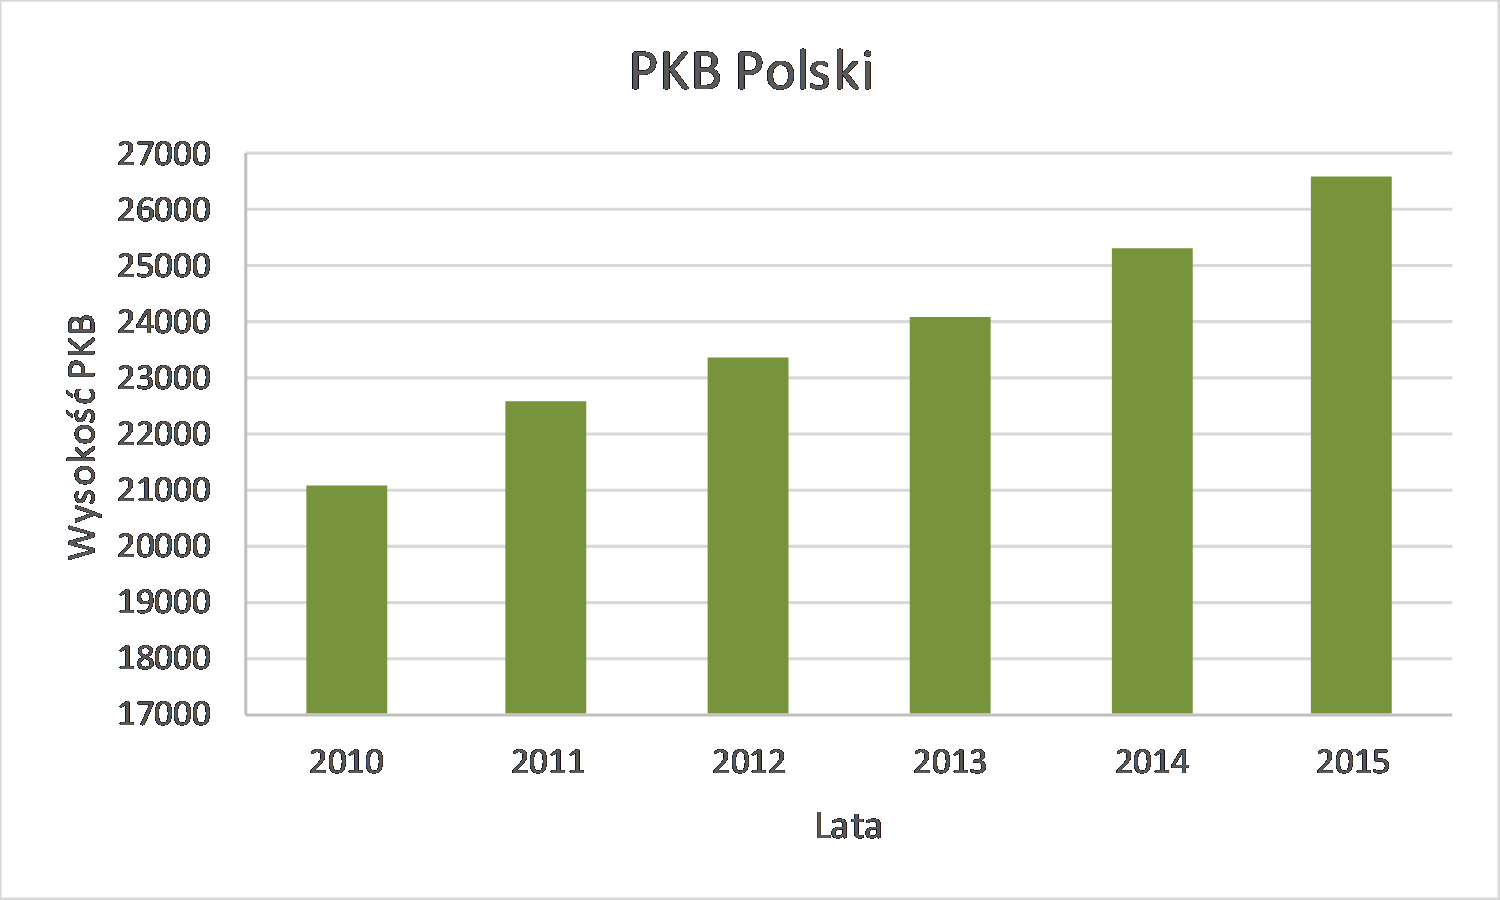
\includegraphics[width=1\textwidth]{ART_Rybka/pkb_polski.png} 
	\caption{Zmiana PKB \textit{per capita} według parytetu siły nabywczej mierzona dolarami międzynarodowymi.
		Źródło: opracowanie własne na podstawie
		\parencite{international_monetary_fund_world_2019a}.
%		\label{ref:RNDl3ypL6FseV}(International Monetary Fund, 2019a).
	}
	\label{fig1:ryb}
\end{figure}


%{\centering
%Rysunek 1. Zmiana PKB per capita według parytetu siły nabywczej mierzona dolarami międzynarodowymi%
%%Warto usunąć z~osi x lata ,,połówkowe'' bo to wygląda dziwacznie
%%nieznany
%%30 sierpnia 2019 15:45
%
%\par}
%
%{\centering
%[[[rysunek\_1]]]
%\par}
%
%źródło: opracowanie własne na podstawie \label{ref:RNDl3ypL6FseV}(International Monetary Fund, 2019a)

Jak wskazuje Rysunek \ref{fig1:ryb}, wartości PKB systematycznie rosły. Średni wzrost wskaźnika PKB w~latach 2010–2015 dla Polski
wynosi 1103,7 dolarów międzynarodowych. Najniższa wartość została odnotowana w~2010 r. Wynosi ona 21083,87 dolarów,
a~najwyższa pochodząca z~2015~r. to 26602,35. 

\begin{figure}[H]
	\centering
	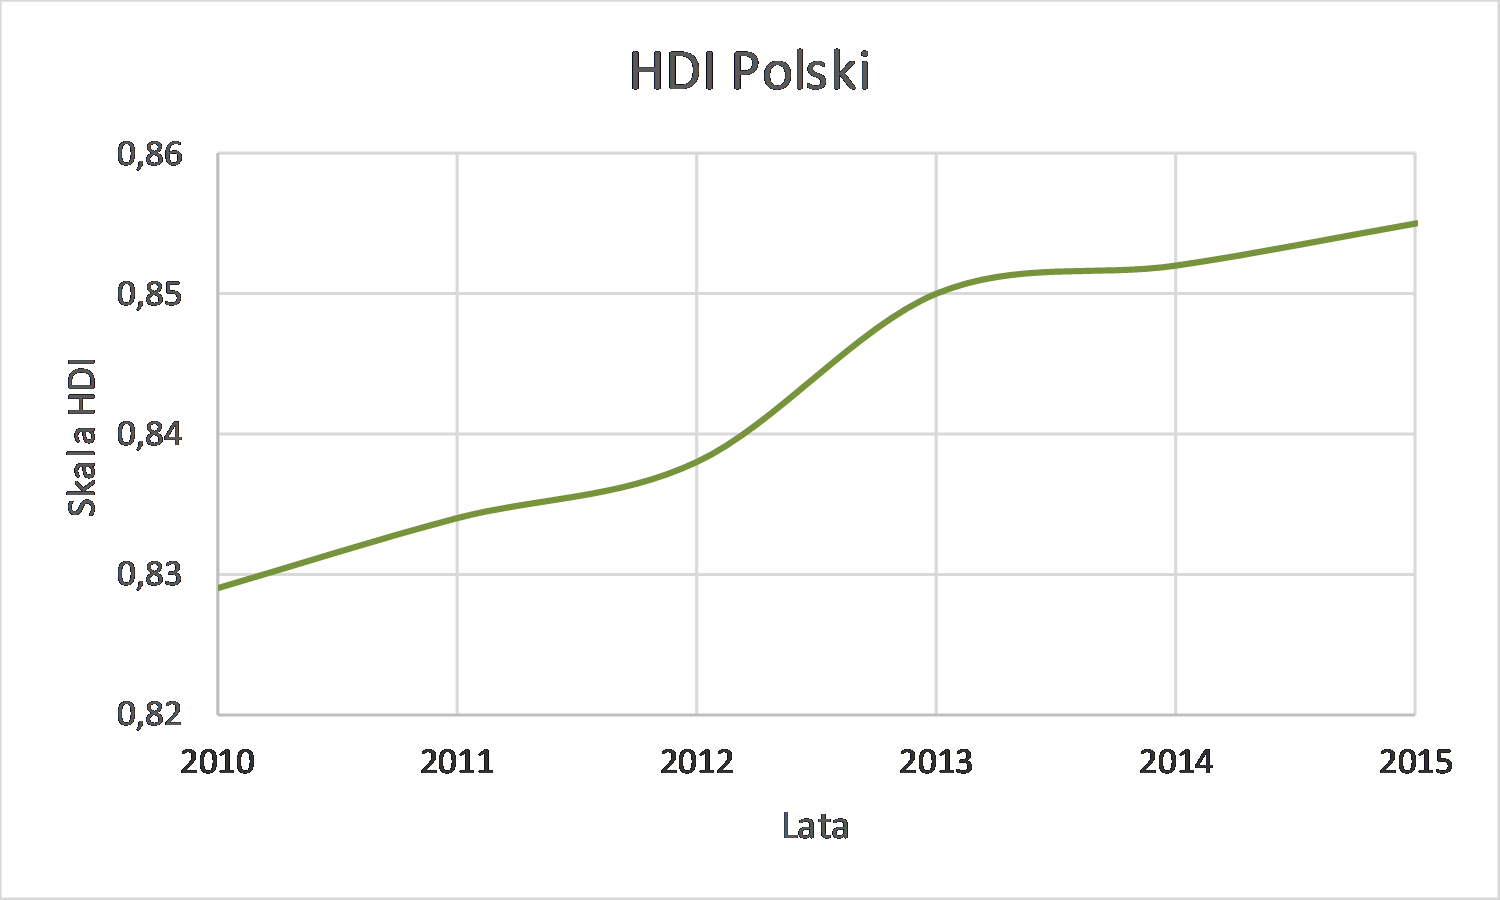
\includegraphics[width=1\textwidth]{ART_Rybka/hdi_polski.png} 
	\caption{Zmiana wartości HDI dla Polski.
		Źródło: opracowanie własne na podstawie
		\parencite{united_nations_development_programme_human_2019}.
%		\label{ref:RNDSuSEh9knxi}(United Nations Development Programme, 2019).
	}
	\label{fig2:ryb}
\end{figure}


%{\centering
%Rysunek 2. Zmiana wartości HDI dla Polski
%\par}
%
%{\centering
%[[[rysunek\_2]]]
%\par}
%
%źródło: opracowanie własne na podstawie \label{ref:RNDSuSEh9knxi}(United Nations Development Programme, 2019)

Wykres liniowy znajdujący się na Rysunku \ref{fig2:ryb} pokazuje zmiany zachodzące w~wartościach wskaźnika HDI. Przez cały okres
badania można zauważyć tendencję wzrostową. Największa zmiana wynosząca 0,012j. zachodzi pomiędzy 2012 a~2013 rokiem.
Średni wzrost wskaźnika HDI dla Polski to 0,0052j. przypadający na jeden rok badanego okresu. Różnica pomiędzy
wartością najwyższą oraz najniższą wynosi 0,03j.

\begin{figure}[H]
	\centering
	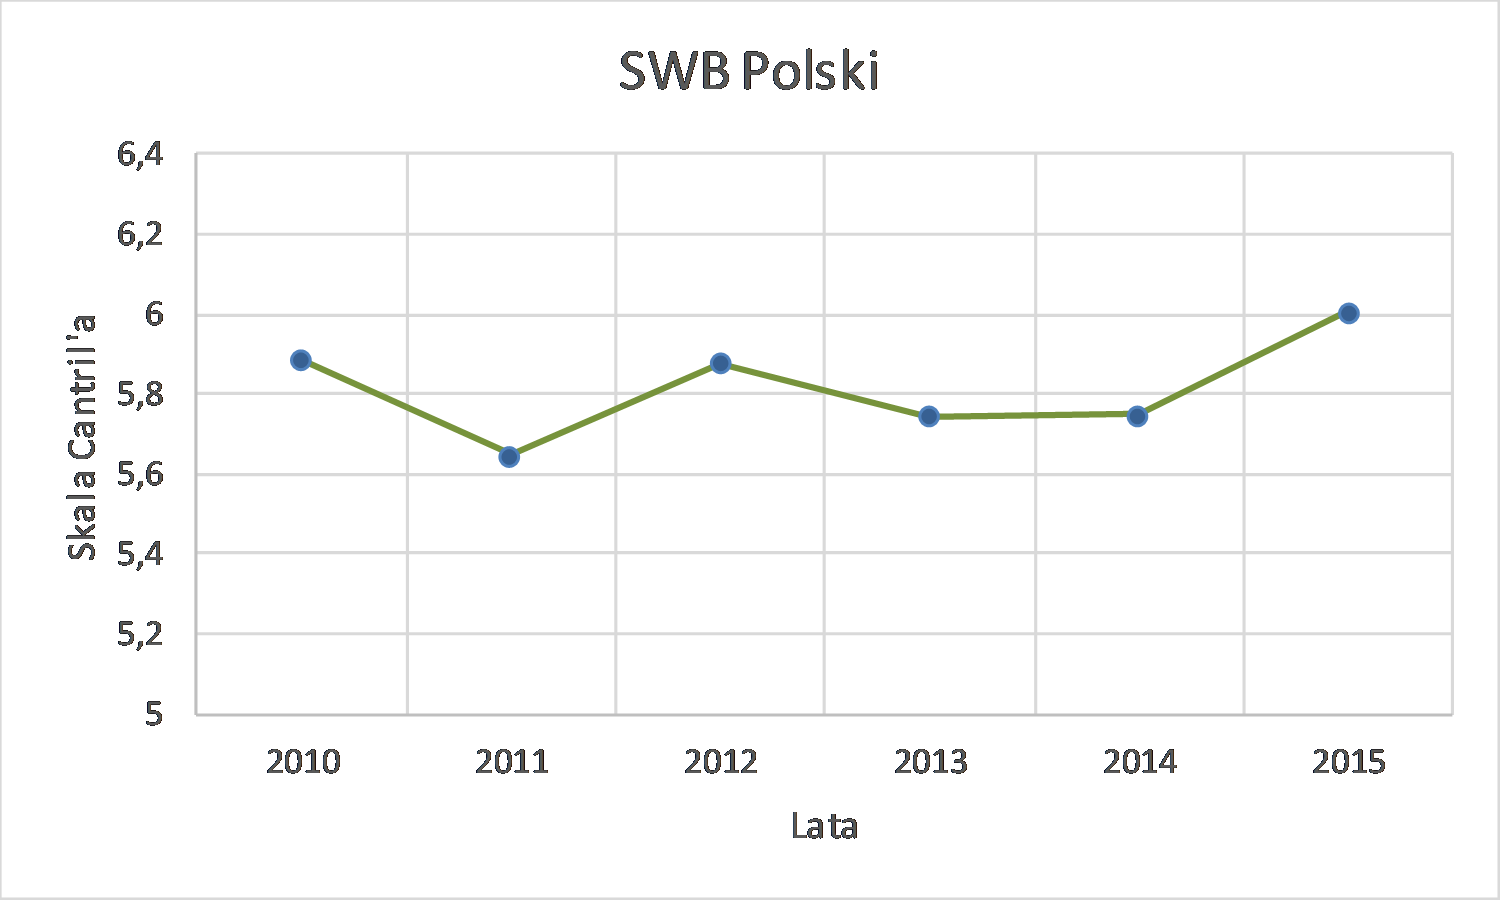
\includegraphics[width=1\textwidth]{ART_Rybka/swb_polski.png} 
	\caption{Zmiana wartości wskaźnika SWB Polski.
		Źródło: opracowanie własne na podstawie
		\parencite{noauthor_world_2018}.
%		\label{ref:RNDWHAJqDwCvX}(World Happiness Report, 2018).
	}
	\label{fig3:ryb}
\end{figure}


%{\centering
%Rysunek 3. Zmiana wartości wskaźnika SWB Polski
%\par}
%
%{\centering
%[[[rysunek\_3]]]
%\par}
%
%źródło: opracowanie własne na podstawie \label{ref:RNDWHAJqDwCvX}(World Happiness Report, 2018)

Na Rysunku \ref{fig3:ryb} została przedstawiona zmiana wartości wskaźnika SWB dla Polski. Jak można zaobserwować, wyniki skali
zmieniały się nieregularnie. W~latach 2010--2011 oraz 2012--2013 zauważalny jest spadek wartości wskaźnika, zaś w~latach
2011--2012 oraz 2013--2015 można spostrzec jego wzrost. Średni wzrost wskaźnika SWB wynosi 0,02j. Różnica pomiędzy
skrajnymi wartościami wynosi 0,36j.

Dla danych uzyskanych przez pomiar wskaźnikami PKB, HDI oraz SWB została przeprowadzona korelacja pomiędzy
poszczególnymi miernikami. Jej wyniki przedstawia poniższa tabela.

\captionsetup[table]{name=Tabela}
\begin{table}[H]
	\begin{tabularx}{\textwidth}{|Y|Y|}
		\hline
		\multicolumn{2}{|c|}{\bfseries Korelacja wskaźników dla Polski}\\\hline
		PKB z~SWB &
		0,32\\\hline
		PKB z~HDI &
		0,95\\\hline
		HDI z~SWB &
		0,21\\\hline
	\end{tabularx}
	
	\caption{Wartości związku pomiędzy poszczególnymi wskaźnikami dla Polski.
		Źródło: opracowanie własne na podstawie
		\parencite{international_monetary_fund_world_2019a,united_nations_development_programme_human_2019,noauthor_world_2018}.
%		\label{ref:RNDJaFcYZDBCr}(International Monetary Fund, 2019a; United Nations
%		Development Programme, 2019; World Happiness Report, 2018).
		}
	\label{tab3:ryb}
\end{table}


%{\centering
%Tabela 3 Wartości związku pomiędzy poszczególnymi wskaźnikami dla Polski
%\par}
%
%\begin{center}
%\tablefirsthead{}
%\tablehead{}
%\tabletail{}
%\tablelasttail{}
%\begin{supertabular}{|m{4.552cm}|m{4.55cm}|}
%\hline
%\multicolumn{2}{|m{9.302cm}|}{\centering{\bfseries Korelacja wskaźników dla Polski}}\\\hline
%\centering PKB z~SWB &
%\centering\arraybackslash 0,32\\\hline
%\centering PKB z~HDI &
%\centering\arraybackslash 0,95\\\hline
%\centering HDI z~SWB &
%\centering\arraybackslash 0,21\\\hline
%\end{supertabular}
%\end{center}
%źródło: opracowanie własne na podstawie \label{ref:RNDJaFcYZDBCr}(International Monetary Fund, 2019a; United Nations
%Development Programme, 2019; World Happiness Report, 2018)

%\enlargethispage{1\baselineskip}

Tabela \ref{tab3:ryb} przedstawiająca korelacje pomiędzy wartościami otrzymanymi przez mierniki wskazuje, że największy związek
zachodzi pomiędzy PKB oraz HDI, który wynosi 0,95 -- oznacza to, że korelacja między nimi jest bardzo silna. Tak
jak w~przypadku danych dla 103 państw, tak wysoki związek pomiędzy danymi może wynikać z~tego, że 1/3 wartości wskaźnika HDI
pozyskiwana jest z~danych dochodu narodowego brutto \textit{per capita}, który jest pochodną PKB. Związek pomiędzy
PKB a~wynikami SWB wyrażany współczynnikiem korelacji Pearsona wynosi 0,32. Jest to korelacja słaba, oznaczająca znikome
powiązanie pomiędzy tymi wskaźnikami. Najmniejszym związkiem statystycznym charakteryzują się mierniki HDI oraz SWB.
Wynosi on 0,21, co jest postrzegane jako bardzo słaba korelacja, lub praktycznie zerowy związek pomiędzy wartościami. 

Niska korelacja pomiędzy PKB i~SWB oraz HDI i~SWB może być związana z~tym, że Polacy nie utożsamiają swojego zadowolenia
z życia z~otrzymywanym dochodem. Według obliczeń przeprowadzonych na podstawie danych pochodzących z~World
Happiness Report wynika, że istnieje wysoka korelacja pomiędzy subiektywnym dobrobytem a~postrzeganym poziomem korupcji
na szczeblu rządowym i~samorządowym oraz w~sektorze prywatnym. Związek statystyczny pomiędzy SWB a~postrzeganym
poziomem korupcji wynosi -0,78, co jest korelacją silną oraz odwrotną. Oznacza to, że wraz ze spadkiem (wzrostem)
korupcji w~rządzie i~sektorze prywatnym wzrasta (spada) zadowolenie z~życia obywateli Polski. Średnia wyników
ankiet z~lat 2010--2015 mówi, że średnio aż 88\% ankietowanych uważa, że korupcja jest rozpowszechniona na szczeblu rządowym oraz
prywatnym
\parencite{noauthor_world_2018}.
%\label{ref:RNDcRU0ppjN4H}(World Happiness Report, 2018).
Zdaniem autora niska zależność pomiędzy PKB a~SWB
może być spowodowana tym, że Polacy mogą czuć się oszukiwani i~bezsilni wobec panujących układów korupcyjnych w~Polsce,
przez co wzrost (spadek) wynagrodzenia nie wiąże się ze wzrostem (spadkiem) poziomu subiektywnego dobrobytu.

%\enlargethispage{1\baselineskip}

Jak zostało przedstawione na
powyższych wykresach, wzrost wartości wskaźnika PKB \textit{per capita} według parytetu siły nabywczej mierzonego dolarami
amerykańskimi oznacza znikomy wzrost poziomu zadowolenia z~życia (SWB) wyrażonego przez Drabinę Cantrila. Najbardziej
skorelowane okazały się PKB oraz HDI. Związek pomiędzy nimi jest bardzo silny.
Wzrost jednego ze wskaźników powoduje wzrost średniej wartości drugiego wskaźnika. Korelacje pomiędzy miernikami
PKB i~SWB oraz HDI i~SWB są bardzo znikome. Może to być spowodowane pozaekonomicznymi czynnikami, które wpływają na
subiektywny dobrobyt mieszkańców Polski.

Drugim krajem przeprowadzonej analizy jest Grecja. To kraj południowo-wschodniej Europy. W~2002 r. Grecja
zrezygnowała ze swojej waluty na rzecz euro, w~2013 r. została zakwalifikowana do grupy krajów rozwijających się, co
stanowiło degradację z~kategorii krajów rozwiniętych. Był to pierwszy przypadek spadku z~grupy dla tego kraju
\parencite{international_monetary_fund_world_2019a}.
%\label{ref:RNDOaa1RXQDzx}(International Monetary Fund, 2019a).
W~2017 r. Grecję zamieszkiwało nieco ponad 10~mln mieszkańców,
w~tym samym roku odnotowano wysokość PKB rzędu 201 mld dolarów amerykańskich. PKB \textit{per capita} w~2017~r. osiągnęło zatem
wartość 18630 USD
\parencite{international_monetary_fund_world_2019b}.
%\label{ref:RNDRQRmi2Olaq}(International Monetary Fund, 2019b).
Kraj ten należy do dużej liczby
międzynarodowych organizacji, m.in. Paktu Północnoatlantyckiego od 1952 r., Unii Europejskiej od 1981 r., Organizacji
Narodów Zjednoczonych od 1945 r., oraz Organizacji Współpracy Gospodarczej i~Rozwoju od 1961 r. 

Grecja znajduje się na 28. miejscu rankingu 103 państw, w~którym pod uwagę brano PKB \textit{per capita} według parytetu siły
nabywczej liczonym dolarami międzynarodowymi. Według ranking wskaźnika rozwoju społecznego zajęła 21., a~pod względem
subiektywnego dobrobytu (SWB) znalazła się na 59. miejscu.

%\enlargethispage{1\baselineskip}

W poniższych tabelach zostanie przeprowadzona analiza wskaźnikowa dla Grecji.


\begin{table}[H]
	\begin{footnotesize}
		\begin{tabularx}{\textwidth}{|Y|Y|Y|Y|Y|Y|Y|}
			\hline
			\multicolumn{7}{|c|}{\bfseries Grecja}\\\hline
			~ &
			2010 &
			2011 &
			2012 &
			2013 &
			2014 &
			2015\\\hline
			{\bfseries SWB} &
			5,840 &
			5,372 &
			5,096 &
			4,720 &
			4,756 &
			5,623\\\hline
			{\bfseries PKB} &
			28961,80 &
			26850,25 &
			25433,14 &
			25194,26 &
			26017,86 &
			26389,71\\\hline
			{\bfseries HDI} &
			0,860 &
			0,858 &
			0,860 &
			0,862 &
			0,865 &
			0,866\\\hline
		\end{tabularx}
	\end{footnotesize}
	
	\caption{Zmiana wartości wskaźników Grecji.
		Źródło: oobliczenia własne na podstawie
		\parencite{international_monetary_fund_world_2019a,united_nations_development_programme_human_2019,noauthor_world_2018}.
%		\label{ref:RNDIkw0V6s683}(International Monetary Fund, 2019a; United Nations
%		Development Programme, 2019; World Happiness Report, 2018).
	}
	\label{tab4:ryb}
\end{table}

%{\centering
%Tabela 4 Zmiana wartości wskaźników Grecji
%\par}
%
%\begin{flushleft}
%\tablefirsthead{}
%\tablehead{}
%\tabletail{}
%\tablelasttail{}
%\begin{supertabular}{|m{3.6139998cm}|m{1.8179998cm}|m{1.977cm}|m{1.977cm}|m{1.9779999cm}|m{1.977cm}|m{1.984cm}|}
%\hline
%\multicolumn{7}{|m{16.525cm}|}{\centering{\bfseries Grecja}}\\\hline
%\centering{\bfseries ~} &
%\centering 2010 &
%\centering 2011 &
%\centering 2012 &
%\centering 2013 &
%\centering 2014 &
%\centering\arraybackslash 2015\\\hline
%\centering{\bfseries SWB} &
%\centering 5,840 &
%\centering 5,372 &
%\centering 5,096 &
%\centering 4,720 &
%\centering 4,756 &
%\centering\arraybackslash 5,623\\\hline
%\centering{\bfseries PKB} &
%\centering 28961,801 &
%\centering 26850,252 &
%\centering 25433,138 &
%\centering 25194,264 &
%\centering 26017,860 &
%\centering\arraybackslash 26389,706\\\hline
%\centering{\bfseries HDI} &
%\centering 0,860 &
%\centering 0,858 &
%\centering 0,860 &
%\centering 0,862 &
%\centering 0,865 &
%\centering\arraybackslash 0,866\\\hline
%\end{supertabular}
%\end{flushleft}
%źródło: obliczenia własne na podstawie \label{ref:RNDIkw0V6s683}(International Monetary Fund, 2019a; United Nations
%Development Programme, 2019; World Happiness Report, 2018)

Tabela \ref{tab4:ryb} pokazuje zmiany wartości wskaźników, jakie zachodziły na przestrzeni sześciu lat dla Grecji. Wskaźniki PKB oraz
SWB wskazują spadek swoich wartości w~latach od 2010 do 2013. Natomiast od 2013 do 2015 roku oba zaczęły wzrastać.
Wskaźnik rozwoju społecznego, oprócz roku 2011, w~którym zauważono spadek, wzrastał. Średnie wartości wskaźników to:

\begin{itemize}
\item SWB -- 5,234,
\item PKB -- 26474,504,
\item HDI -- 0,862.
\end{itemize}

%\enlargethispage{1\baselineskip}

\begin{figure}[H]
	\centering
	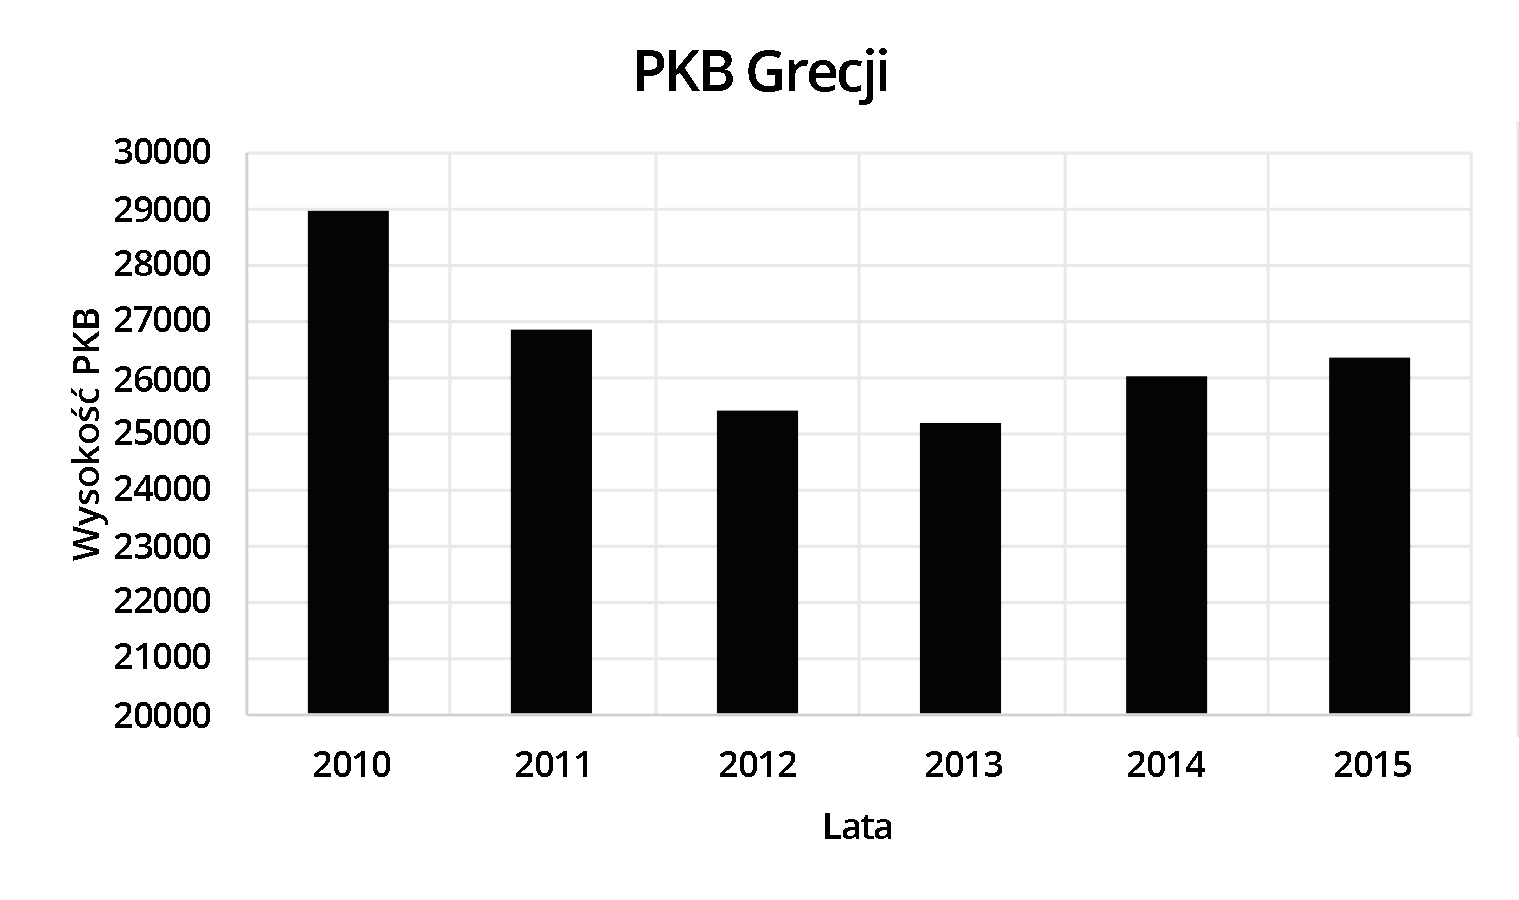
\includegraphics[width=1\textwidth]{ART_Rybka/pkb_grecji.png} 
	\caption{Zmiana PKB Grecji \textit{per capita} według parytetu siły nabywczej mierzona dolarami międzynarodowymi.
		Źródło: opracowanie własne na podstawie
		\parencite{international_monetary_fund_world_2019a}.
%		\label{ref:RND6yFA9J8VHO}(International Monetary Fund, 2019a).
	}
	\label{fig4:ryb}
\end{figure}

%{\centering
%Rysunek 4 Zmiana PKB per capita według parytetu siły nabywczej mierzona dolarami międzynarodowymi Grecji
%\par}
%
%{\centering
%[[[rysunek\_4]]]
%\par}
%
%źródło: opracowanie własne na podstawie \label{ref:RND6yFA9J8VHO}(International Monetary Fund, 2019a)

W zmianie wskaźnika PKB dla Grecji można zauważyć dwie tendencje. Jedna malejąca rozpoczynająca się w~2010 roku,
a kończąca się w~roku 2013, oraz wzrostowa, która początek ma w~2013~r. do 2015~r. PKB swoją największą wartość osiągnęło
w 2010 r., wyniosła ona 28961,801 dolarów międzynarodowych oraz najniższą w~2013~r. wynoszącą 25194,264. Średnia zmiana
wartości PKB wyniosła 514,419 dolarów. Różnica pomiędzy najwyższym i~najniższym odnotowanym PKB wynosi 3767,537 dolarów.


\begin{figure}[h]
	\centering
	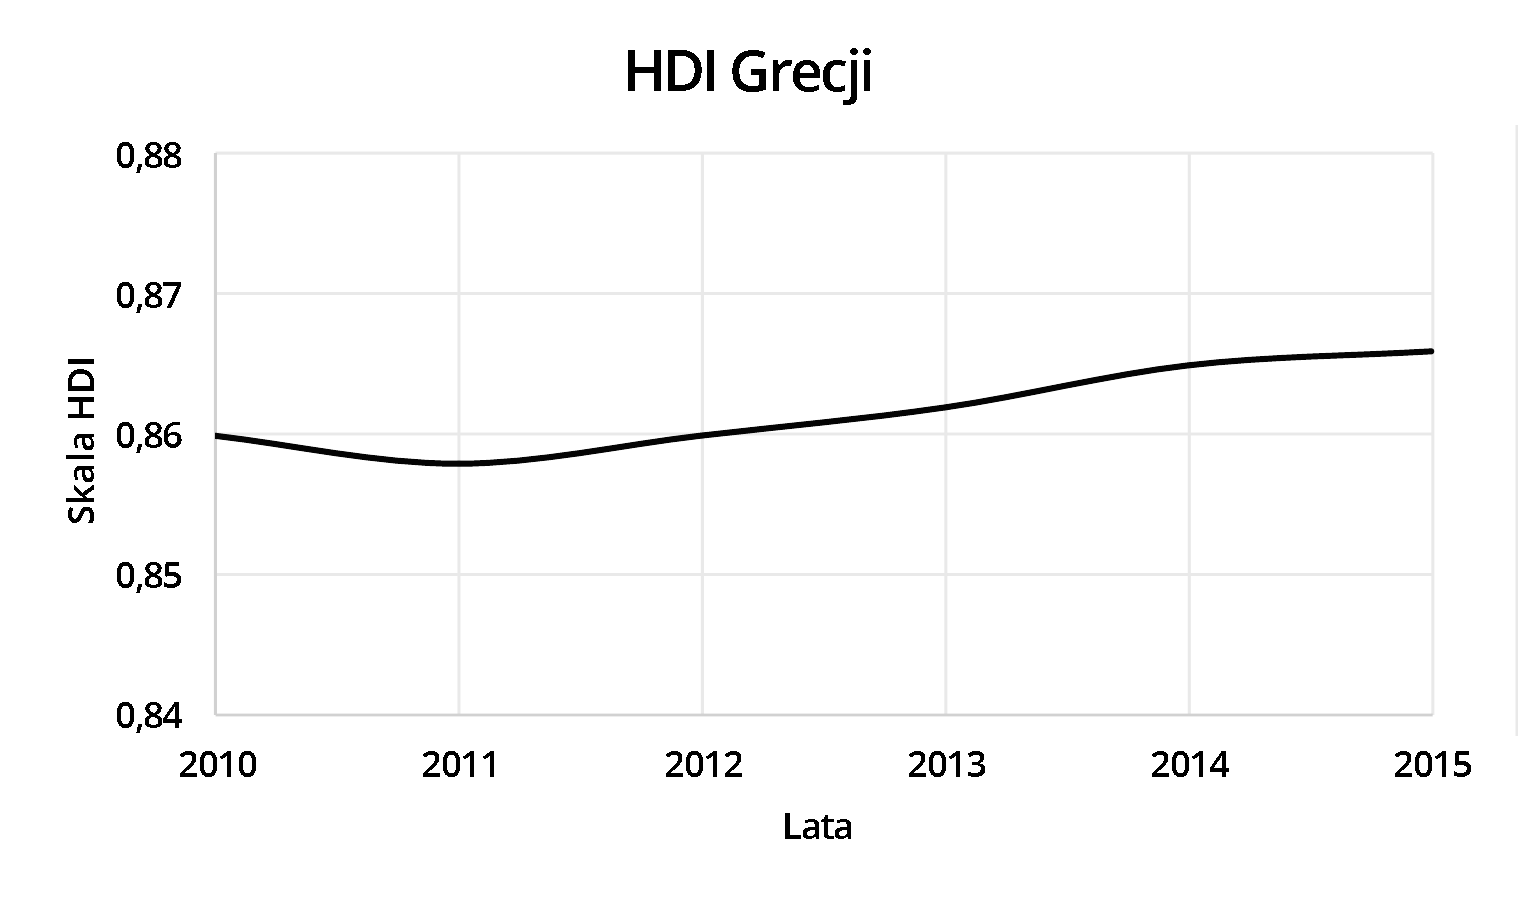
\includegraphics[width=1\textwidth]{ART_Rybka/hdi_grecji.png} 
	\caption{Zmiana wartości HDI Grecji.
		Źródło: opracowanie własne na podstawie
		\parencite{united_nations_development_programme_human_2019}.
%		\label{ref:RNDRvQ01uztWh}(United Nations Development Programme, 2019).
	}
	\label{fig5:ryb}
\end{figure}

%{\centering
%Rysunek 5 Zmiana wartości HDI Grecji
%\par}
%
%{\centering
%[[[rysunek\_5]]]
%\par}
%
%źródło: opracowanie własne na podstawie \label{ref:RNDRvQ01uztWh}(United Nations Development Programme, 2019)

Linia wskazująca zmiany HDI ulega niewielkim zmianom w~ciągu badanego okresu. Oprócz spadku w~roku 2011 tendencja
wskaźnika jest wzrastająca. Najwyższy punkt funkcja osiągnęła w~roku 2015 i~wyniosła 0,866, a~najniższy z~2011 roku
wyniósł 0,858. Różnica pomiędzy nimi wynosi 0,008. Średni wzrost wskaźnika HDI wyniósł 0,0012. 

\begin{figure}[h]
	\centering
	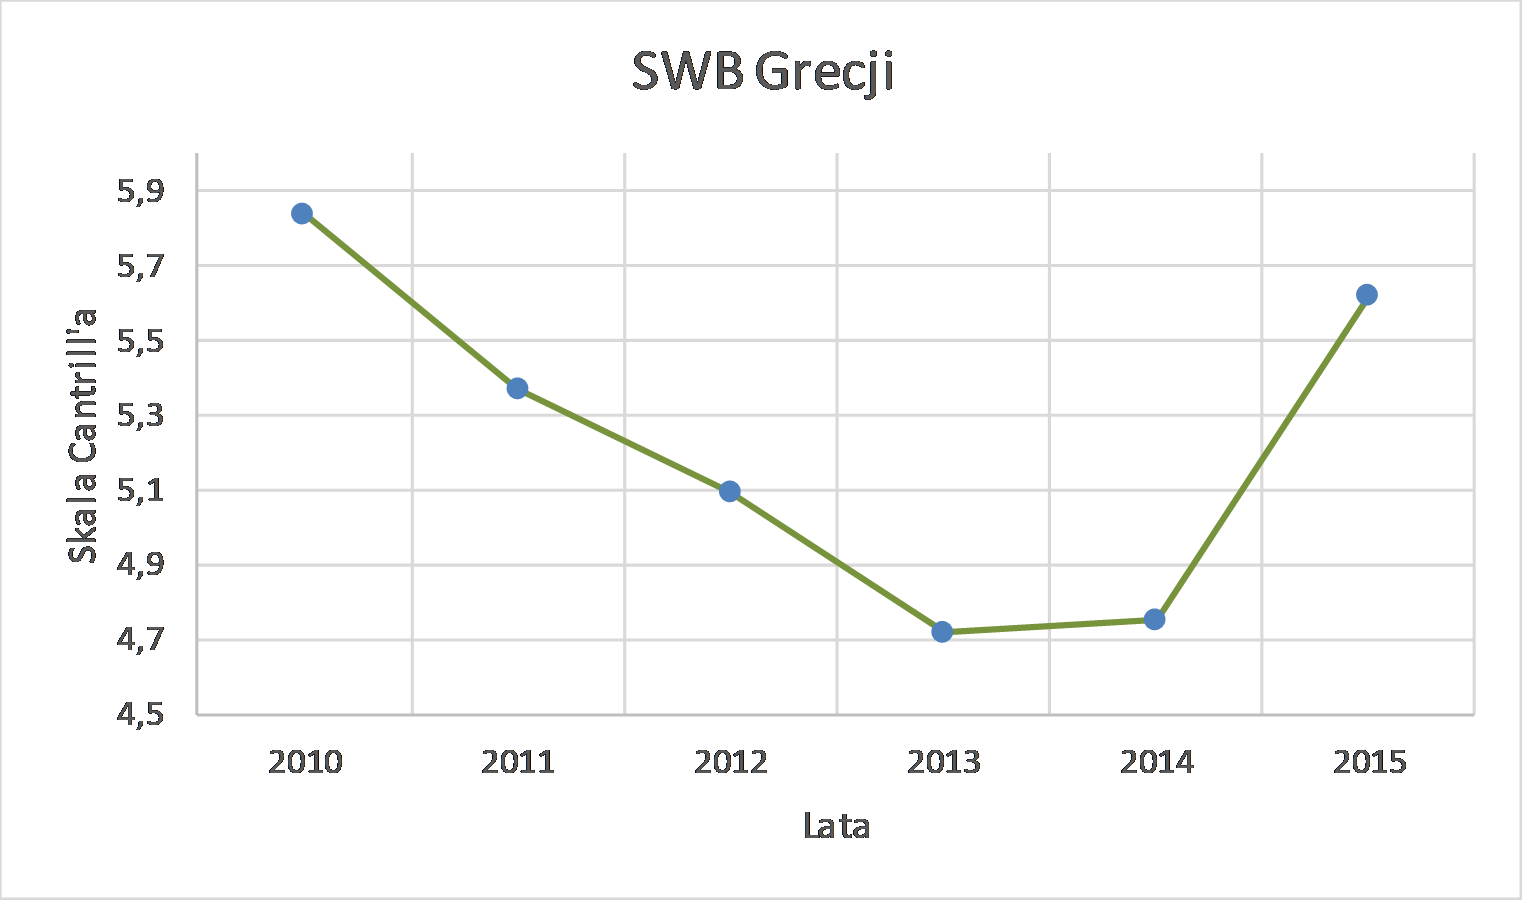
\includegraphics[width=1\textwidth]{ART_Rybka/swb_grecji.png} 
	\caption{Zmiana wartości SWB Grecji.
		Źródło: opracowanie własne na podstawie
		\parencite{noauthor_world_2018}.
%		\label{ref:RNDB7u1qcEsSx}(World Happiness Report, 2018).
	}
	\label{fig6:ryb}
\end{figure}


%{\centering
%Rysunek 6 Zmiana wartości SWB Grecji
%\par}
%
%{\centering
%[[[rysunek\_6]]]
%\par}
%
%źródło: opracowanie własne na podstawie \label{ref:RNDB7u1qcEsSx}(World Happiness Report, 2018)

Wykres łączący punkty wartości SWB wskazuje podział na dwa okresy: spadku oraz wzrostu. Pierwszy z~nich zauważalny jest
na przestrzeni lat 2010--2013. Drugi to okres wzrostu występujący w~latach 2013--2015. Najwyższy punkt wykresu przypada
na rok 2010 i~wynosi 5,84. Najniższy został odnotowany w~roku 2013, który wskazuje na wartość 4,72. Różnica pomiędzy
najwyższym i~najniższym punktem wynosi 1,12.  Największy wzrost wartości został odnotowany pomiędzy 2014 i~2015 rokiem
i~wyniósł 0,866. Średni spadek wartości SWB Grecji w~badanym okresie wyniósł 0,043.

\captionsetup[table]{name=Tabela}
\begin{table}[H]
	\begin{tabularx}{\textwidth}{|Y|Y|}
		\hline
		\multicolumn{2}{|c|}{\bfseries Korelacja wskaźników dla Grecji}\\\hline
		PKB z~SWB &
		0,82\\\hline
		PKB z~HDI &
		-0,29\\\hline
		HDI z~SWB &
		{}-0,19\\\hline
	\end{tabularx}
	
	\caption{Wartości związku pomiędzy wskaźnikami Grecji.
		Źródło: obliczenia własne na podstawie
		\parencite{international_monetary_fund_world_2019a,united_nations_development_programme_human_2019,noauthor_world_2018}.
%		\label{ref:RNDUidV4ndp13}(International Monetary Fund, 2019a; United Nations
%		Development Programme, 2019; World Happiness Report, 2018).
	}
	\label{tab5:ryb}
\end{table}


%{\centering
%Tabela 5 Wartości związku pomiędzy wskaźnikami Grecji
%\par}
%
%\begin{center}
%\tablefirsthead{}
%\tablehead{}
%\tabletail{}
%\tablelasttail{}
%\begin{supertabular}{|m{5.3cm}|m{3.441cm}|}
%\hline
%\multicolumn{2}{|m{8.941cm}|}{\centering Grecja}\\\hline
%\centering PKB z~SWB &
%\centering\arraybackslash 0,82\\\hline
%\centering PKB z~HDI &
%\centering\arraybackslash {}-0,29\\\hline
%\centering HDI z~SWB &
%\centering\arraybackslash {}-0,19\\\hline
%\end{supertabular}
%\end{center}
%źródło: obliczenia własne na podstawie \label{ref:RNDUidV4ndp13}(International Monetary Fund, 2019a; United Nations
%Development Programme, 2019; World Happiness Report, 2018)

Tabela \ref{tab5:ryb} wskazuje na wartości związku pomiędzy poszczególnymi wskaźnikami. Największa korelacja zachodzi pomiędzy
wskaźnikami PKB oraz SWB, która wynosi 0,82. Jest to związek silny, a~przez niektóre źródła uznawany za bardzo silny.
Wynika z~niego, że wraz ze wzrostem wartości jednego wskaźnika następuje wzrost średniej wartości drugiego. Najniższą,
ujemną korelacją odznaczyły się mierniki HDI oraz SWB, która wyniosła -0,19. Jest to słaby związek pomiędzy danymi.
Podobną sytuację można zauważyć pomiędzy wskaźnikami PKB oraz HDI, dla której korelacja wyniosła -0,29. Dla obu
wartości wzrost (spadek) jednego wskaźnika oznaczał spadek (wzrost) drugiego. 

Tym, co najsilniej przykuwa uwagę, jest zadziwiająco wysoka korelacja pomiędzy PKB oraz SWB. Wartość
związku pomiędzy nimi jest silna. Oznacza to, że wzrost (spadek) zamożności obywateli
Grecji wiązał się ze wzrostem (spadkiem) ich subiektywnego dobrobytu. Taka sytuacja może być spowodowana kryzysem
gospodarczym, który panuje w~Grecji, oraz z~nastrojami mieszkańców. Jak można zauważyć analizując wykresy PKB oraz SWB,
oba wskaźniki odnotowały spadki i~wzrosty dokładnie w~tych samych latach. Także skrajne wartości tych wskaźników
przypadały na ten sam okres. Zadziwiająca jest także sytuacja mająca miejsce pomiędzy wskaźnikami PKB oraz HDI. Nie
tylko korelacja między nimi jest słaba, to na dodatek jest ona odwrotna, co oznacza, że wraz ze wzrostem (spadkiem)
wartości jednego ze wskaźników związany był spadek (wzrost) wartości drugiego wskaźnika. Jest to sytuacja nietypowa,
ponieważ dochód narodowy brutto \textit{per capita} będący pochodną wskaźnika PKB jest częścią HDI. Najniższa korelacja
wystąpiła pomiędzy wskaźnikami HDI oraz SWB, która odznaczała się słabym związkiem. 

Autor pracy przeprowadził obliczenia dotyczące korelacji pomiędzy zadowoleniem z~życia, a~poziomem wskaźnika Giniego.
Wynika z~nich, że istnieje bardzo silny związek pomiędzy tymi dwiema sferami, ponieważ wskaźnik korelacji Pearsona
wynosi aż -0,88. Jest to korelacja odwrotna, z~której wynika, że wraz ze wzrostem (spadkiem) nierówności dochodowych
spada (wzrasta) subiektywne zadowolenie z~życia Greków. Ta sytuacja może być związana z~panującym w~tych
latach w~Grecji kryzysem gospodarczym. Druga wysoka korelacja, która wynosi 0,74, jest zauważalna pomiędzy subiektywnym
dobrobytem a~wolnością podejmowania życiowych decyzji
\parencite{noauthor_world_2018}.
%\label{ref:RNDaAxMI6IUZa}(World Happiness Report, 2018).
Oznacza
to, że dla Greków ważną kwestią wpływającą na ich subiektywne zadowolenie może być wolność w~podejmowaniu decyzji
związanych z~własnym życiem.

Powyższe badania potwierdzają hipotezę, która mówi, że wzrost dobrobytu ekonomicznego nie zawsze wiąże się
ze wzrostem subiektywnego dobrobytu. Obliczenia dotyczące wszystkich 103. państw pokazują także, że największy związek
występuje pomiędzy dobrobytem ekonomicznym oraz ogólnym. Hipoteza zakładała także występowanie większego związku
pomiędzy dobrobytem ogólnym i~subiektywnym niż dobrobytem ogólnym oraz ekonomicznym, lecz przeprowadzone obliczenia jej
zaprzeczają.

\section{Zakończenie}
Tematem przewodnim pracy było wskazanie różnorodności teorii dobrobytu, przedstawienie wskaźników
umożliwiających ich pomiar oraz analiza zależności statystycznych pomiędzy trzema rodzajami dobrobytu (ekonomicznym,
ogólnym oraz subiektywnym) obliczonymi przez wskaźniki PKB, HDI oraz SWB. Z~opracowania wynika, że istnieje bardzo
szeroka gama teorii oraz koncepcji związanych z~dobrobytem, które czasami się wykluczają. Czytelnik może także się
dowiedzieć, że pod jednym hasłem -- dobrobyt -- w~polskiej literaturze kryją się dwa, różne od siebie zjawiska, czyli
dobrobyt ekonomiczny (\textit{welfare)} oraz dobrobyt ogólny (\textit{well-being}). Najważniejszym wnioskiem
płynącym z~opracowania jest to, że związki pomiędzy dobrobytem ekonomicznym a~ogólnym reprezentowanym kolejno przez PKB
oraz HDI są bardzo silne, a~związki pomiędzy dobrobytem ekonomicznym i~subiektywnym zadowoleniem z~życia (SWB
obliczonym za pomocą drabiny Cantrila) oraz dobrobytem ogólnym i~subiektywnym są znikome. Jednak jak pokazują analizy
szczegółowe przeprowadzone na dwóch krajach Unii Europejskiej -- Polsce oraz Grecji -- związki te nie zawsze są silne. 

Przeprowadzone badanie wskazuje jedynie na zależność pomiędzy wartościami dobrobytu poszczególnych krajów.
Związek także nie uwzględnia zależności przyczynowej, tylko obrazuje, że dane zjawiska zachodzą obok
siebie. Ukazuje to jedynie, że dane zjawiska mają miejsce, lecz badania nie wskazują konkretnie przyczyn ich
występowania. Aby wytłumaczyć zaistnienie pewnych zależności, można prześledzić sytuację społeczno-ekonomiczną
mieszkańców danych państw, w~celu poznania przyczyn. 

Autor pracy uważa, że przyszłe badania nad zjawiskiem dobrobytu powinny być prowadzone we współpracy z~przedstawicielami
wielu dziedzin naukowych w~celu zbadania aspektów mogących wpływać na dobrobyt. W~szczególności rekomenduje współpracę
nauk psychologicznych z~ekonomicznymi w~celu dokładnego zbadania dobrobytu subiektywnego.

\end{artplenv}\label{rybka-stop}

